% Options for packages loaded elsewhere
\PassOptionsToPackage{unicode}{hyperref}
\PassOptionsToPackage{hyphens}{url}
\PassOptionsToPackage{dvipsnames,svgnames*,x11names*}{xcolor}
%
\documentclass[
  fontsize=10pt,
  a4paper,
]{scrartcl}
\usepackage{amsmath,amssymb}
\usepackage{lmodern}
\usepackage{iftex}
\usepackage[T1]{fontenc}
\usepackage[utf8]{inputenc}
\usepackage[english]{babel}
\usepackage{textcomp} % provide euro and other symbols
\usepackage{longtable}
\usepackage{url}
\usepackage{multirow}
\usepackage[english,verbose]{layout}
\usepackage{float}
\floatplacement{figure}{H}
\usepackage[]{biblatex}
\addbibresource{biblio.bib}
\usepackage{multirow}
\usepackage{enumitem}
\usepackage{exercises}
\usepackage{xcolor}

\usepackage{mypythonstyle}


%--------------------------------------------------------------------
% For MC questions
%--------------------------------------------------------------------
\newcounter{choice}
\renewcommand\thechoice{\Alph{choice}}
\newcommand\choicelabel{\thechoice.}

\newenvironment{choices}%
  {\list{\choicelabel}%
     {\usecounter{choice}\def\makelabel##1{\hss\llap{##1}}%
       \settowidth{\leftmargin}{W.\hskip\labelsep\hskip 2.5em}%
       \def\choice{%
         \item
       } % choice
       \labelwidth\leftmargin\advance\labelwidth-\labelsep
       \topsep=0pt
       \partopsep=0pt
     }%
  }%
  {\endlist}

\newenvironment{oneparchoices}%
  {%
    \setcounter{choice}{0}%
    \def\choice{%
      \refstepcounter{choice}%
      \ifnum\value{choice}>1\relax
        \penalty -50\hskip 1em plus 1em\relax
      \fi
      \choicelabel
      \nobreak\enskip
    }% choice
    % If we're continuing the paragraph containing the question,
    % then leave a bit of space before the first choice:
    \ifvmode\else\enskip\fi
    \ignorespaces
  }%
  {}

%--------------------------------------------------------------------
% Use upquote if available, for straight quotes in verbatim environments
\IfFileExists{upquote.sty}{\usepackage{upquote}}{}
\IfFileExists{microtype.sty}{% use microtype if available
  \usepackage[]{microtype}
  \UseMicrotypeSet[protrusion]{basicmath} % disable protrusion for tt fonts
}{}
\makeatletter
\@ifundefined{KOMAClassName}{% if non-KOMA class
  \IfFileExists{parskip.sty}{%
    \usepackage{parskip}
  }{% else
    \setlength{\parindent}{0pt}
    \setlength{\parskip}{6pt plus 2pt minus 1pt}}
}{% if KOMA class
  \KOMAoptions{parskip=half}}
\makeatother

\IfFileExists{xurl.sty}{\usepackage{xurl}}{} % add URL line breaks if available
\IfFileExists{bookmark.sty}{\usepackage{bookmark}}{\usepackage{hyperref}}
%--------------------------------------------------------------------

\hypersetup{
  pdftitle={Python},
  pdfauthor={Vos, Tanja},
  pdflang={es-ES},
  pdfsubject={},
  pdfkeywords={},
  colorlinks=true,
  linkcolor={Maroon},
  filecolor={Maroon},
  citecolor={Blue},
  urlcolor={Blue}}
\urlstyle{same} % disable monospaced font for URLs

\usepackage[left=2.5cm,right=2.5cm,top=3cm,bottom=3cm]{geometry}
\usepackage{listings}
\newcommand{\passthrough}[1]{#1}
\usepackage{longtable,booktabs,array}
\usepackage{calc} % for calculating minipage widths
% Correct order of tables after \paragraph or \subparagraph
\usepackage{etoolbox}
\makeatletter
\patchcmd\longtable{\par}{\if@noskipsec\mbox{}\fi\par}{}{}
\makeatother

% Allow footnotes in longtable head/foot
\IfFileExists{footnotehyper.sty}{\usepackage{footnotehyper}}{\usepackage{footnote}}
\makesavenoteenv{longtable}
% Make links footnotes instead of hotlinks:
%\DeclareRobustCommand{\href}[2]{#2\footnote{\url{#1}}}
\setlength{\emergencystretch}{3em} % prevent overfull lines
\providecommand{\tightlist}{%
  \setlength{\itemsep}{0pt}\setlength{\parskip}{0pt}}
\setcounter{secnumdepth}{5}
\usepackage{chngcntr}

%Make framed environments
\usepackage{mdframed}
\usepackage{fvextra}
\setkeys{Gin}{width=\maxwidth,height=\maxheight,keepaspectratio}
\DefineVerbatimEnvironment{Highlighting}{Verbatim}{breaklines,commandchars=\\\{\}}

\newenvironment{definition}%
  {\begin{mdframed}[skipabove=10pt,skipbelow=10pt,backgroundcolor=blue!10]}%
  {\end{mdframed}}

\newenvironment{highlights}%
  {\begin{mdframed}[skipabove=10pt,skipbelow=10pt,backgroundcolor=lightgray]}%
  {\end{mdframed}}

\newenvironment{todo}%
  {\begin{mdframed}[skipabove=10pt,skipbelow=10pt,backgroundcolor=yellow!20]}%
  {\end{mdframed}}
  
\newenvironment{remark}%
  {\begin{mdframed}[skipabove=10pt,skipbelow=10pt,backgroundcolor=blue!20]}%
  {\end{mdframed}}  

\newenvironment{feedback}%
  {\begin{mdframed}[skipabove=10pt,skipbelow=10pt,backgroundcolor=orange!20]}%
  {\end{mdframed}}

\newenvironment{domainTILEd}%
  {\begin{mdframed}[skipabove=10pt,skipbelow=10pt,backgroundcolor=green!20]}%
  {\end{mdframed}}  



\newenvironment{howTILEd}%
  {\begin{mdframed}[skipabove=10pt,skipbelow=10pt,backgroundcolor=pink!40]}%
  {\end{mdframed}}



\renewenvironment{abstract}{%
\vspace*{0.3cm}
  \hfill\begin{minipage}{\textwidth}
  \rule{\textwidth}{1pt}}
  {\par\noindent\rule{\textwidth}{1pt}\end{minipage}}  

\newcommand\respuesta[1]{}
\newcommand\solucion[1]{}
\lstnewenvironment{pythonrespuesta}[1][]{}{}
\newcommand\respuestared[0]{}


%%%%%%%%%%%%%%%%%%%%%%%%%%%%%%%%%%%%%%%%%%%%%%%%
%%%%%%%%%%%% TITLE
\title{TILEd Python exercises}
\usepackage{etoolbox}
\makeatletter
\providecommand{\subtitle}[1]{% add subtitle to \maketitle
  \apptocmd{\@title}{\par {\large #1 \par}}{}{}
}
\makeatother
\subtitle{Test Informed Learning with Examples: exercises in Python}
\author{Tanja E.J. Vos}
\date{\today}
%%%%%%%%%%%%%%%%%%%%%%%%%%%%%%%%%%%%%%%%%%%%%%%%

\usepackage{graphicx}




\begin{document}
\maketitle
\begin{abstract}
Python exercises used at the UPV for first year programming courses that have been adapted by using Test Informed Learning with Examples (TILE) to integrate testing in programming education without it costing (much) more time. The coloured boxes indicate how they were TILEd.

\begin{domainTILEd}
This colour box explains a TILE in the \textbf{test domain}.
\end{domainTILEd}

\begin{howTILEd}
This colour box explains a TILE related to \textbf{test runs}
and/or \textbf{test cases}.
\end{howTILEd}
\end{abstract}

\hypertarget{boletin2}{%
\section{Variables, assignments, expressions, basic types}\label{section.var-assign-expr-types}}

\begin{enumerate}
%\setlength{\itemindent}{1.5cm}

\item Most of the programs that we implement:
\begin{enumerate}
\item obtain input data (for example through the keyboard),
\item do something with this data (for example perform some type of computation)
\item display the result as an output (for example on the screen).
\end{enumerate}

Sometimes the combination keyboard/screen is known by the name of the {\em console}, with which both are indistinctly identified.


1. Input data entry is carried out by using the instruction 
\verb+input+ such as in the following example:
\begin{Verbatim}[frame=single]
     n = int(input("Enter a number: "))
\end{Verbatim}
Using this instruction we ask the user for a number through the keyboard. Obviously, this data will have to be stored somewhere in memory, that is, in a variable. The previous instruction indicates that the data entered by the user will be interpreted as an integer (\verb+int+) and will be stored in the variable \verb+n+.


2. Calculate the square of the given number is an example of a computation:

\begin{Verbatim}[frame=single]
     square = n * n
\end{Verbatim}
The previous instruction calculates the square on \verb+n+ and stores the result in the variable \verb+square+.

3. Displaying data is done by using the instruction 
\verb+print+ such as in the following example:

\begin{Verbatim}[frame=single]
     print("The square is", square)
\end{Verbatim}

When we test this program by executing it in the console, we can obtain for example:
\begin{Verbatim}[frame=single, label={\em example test execution of the program}]
>>> %Run 
  Enter a number: 5
  The square is 25
\end{Verbatim}
Note that the program must work whatever has been the number entered by the user. When we write programs with which we can interact through the console, we can test our program by entering test input data through the keyboard en checking the resulting output on the screen.
To test our program to see whether is also works for other numbers, we could execute the following tests through the console:

\begin{Verbatim}[frame=single, label={\em do more tests}]
>>> %Run 
Enter a number: 0
The square is 0
>>> %Run 
Enter a number: -6
The square is 36
>>> %Run 
Enter a number: 1000000
The square is 1000000000000
\end{Verbatim}

\begin{howTILEd}
UnTILEd this exercise said: When executing this program in the console, the user will give input through the keyboard en the results will be shown on the screen

When we TILE the exercise, instead of just saying that we can execute programs through the console, we say we can {\em test} our program this way like we do above. This way we also introduce the students with the terminology:

\begin{itemize}
    \item test your program
    \item test input
    \item checking the resulting output
\end{itemize}

Then with sample executions we invite then to do more tests.
And all of this in one of the very first exercises.
\end{howTILEd}


\item Given two variables \verb+a+ and \verb+b+, write a Python program that allows the user to enter two values for them, swap their values and display them on the
screen. The execution of the program should result in the following:
\begin{Verbatim}[frame=single, label={\em example test execution of the program}]
>>> %Run
  Enter the value of the variable a: 4
  Enter the value of the variable b: 2
  The value of a is 2
  The value of b is 4
\end{Verbatim}
Assuming that 4 and 2 are the values entered by the user. This should work for any pair of user-entered values.

Execute tests through the console and check the output. Does your program work for negative numbers? Does it work for strings? Does it work for characters? Does it work for reals? Can \verb+a+ and \verb+b+ have different types? Should your program work for all these cases?

\begin{howTILEd}
This exercise was TILEd by adding the last paragraph. We explicitly ask the students to test for different types of values. Most students, because of the example execution convert the user input to int, but that is not necessary for the swapping, anything can be swappped. Asking them to test with all kinds of values makes them aware of the assumptions they made when reading the exercises and hence how testing is good to find errors.
\end{howTILEd}



\item Make a program in Python that receive values for three variables
\verb+a+, \verb+b+ and \verb+c+, and interchange their values as follows:
\begin{itemize}
\item \verb+b+ takes the value of \verb+a+, 
\item \verb+c+ takes the value of \verb+a+, and
\item \verb+a+ takes the value of \verb+c+.
\end{itemize}
This must be done WITHOUT using
auxiliary variables, that is, additional helper variables that are not a, b or c, and are used to store some values.

Execute tests through the console and check the output. Does your program work for negative numbers? Does it work for characters? Does it work for reals? Can \verb+a+, \verb+b+ and \verb+c+ have different types? Should your program work for all these cases?


\begin{howTILEd}
This exercise was TILEd by adding the last paragraph. We explicitly ask the students to test for different types of values. Most students, because of the example execution convert the user input to int, but that is not necessary for the swapping, anything can be swappped. Asking them to test with all kinds of values makes them aware of the assumptions they made when reading the exercises and hence how testing is good to find errors.
\end{howTILEd}


\item The expressions on the right of the assignment can be all complex that we want. Implement a program that reads two real numbers, calculates and prints their sum ({\tt +}), subtraction ({\tt -}), product (\verb+*+) and
division (\verb+/+). 

\begin{Verbatim}[frame=single, label={\em example test execution of the program}]
>>> %Run 
  Enter a real number: 2.5
  Enter another real number: 34.903
  The sum is: 37.403
  The subtraction is: -32.403
  The product is: 87.2575
  The division is: 0.07162708076669627
>>> %Run 
  Enter a real number: 0
  Enter another real number: 4
  The sum is: 4.0
  The subtraction is: -4.0
  The product is: 0.0
  The division is: 0.0
>>> %Run 
  Enter a real number: 2000
  Enter another real number: 45.88
  The sum is: 2045.88
  The subtraction is: 1954.12
  The product is: 91760.0
  The division is: 43.59197907585004
\end{Verbatim}

What happens when you test your programs with two zeros? Why does that happen? What could we do about that? 

\begin{howTILEd}
TILEd by adding example test executions for them to test.
\end{howTILEd}

\item Implement a program that reads two integer numbers, calculates and prints their addition, subtraction, product, division and modulus or remainder (\verb+%+). 

\begin{Verbatim}[frame=single, label={\em example test execution of the program}]
>>> %Run 
  Enter a integer number: 4
  Enter another integer number: 6
  The sum (4 + 6) is:  10
  The subtraction (4 - 6) is:  -2
  The product (4 * 6) is:  24
  The division (4/6) is:  0.6666666666666666
  The modulus or remainder (4 % 6) is:  4
>>> %Run 
  Enter a integer number: 0
  Enter another integer number: -100
  The sum (0 + -100) is:  -100
  The subtraction (0 - -100) is:  100
  The product (0 * -100) is:  0
  The division (0 / -100) is:  0
  The modulus or remainder (4 % -100) is:  0
\end{Verbatim}

\begin{howTILEd}
TILEd by adding example test executions for them to test.
\end{howTILEd}

\item Implement a program that calculates the temperature in degrees Celsius from the temperature in degrees Fahrenheit.
The formula is as follows:
\begin{displaymath}
  C = \frac{5}{9}(F-32)\;.
\end{displaymath} 
The input to the program is degrees Fahrenheit introduced by the user. We will save this value in a variable, for example \verb+F+. Then, the program calculates the expression given by the formula and stores the result in another variable, for example \verb+C+. The last step will consist of printing the result for the user.

\begin{Verbatim}[frame=single, label={\em example test execution of the program}]
>>> %Run 
  Enter the degrees Fahrenheit: 84
  84.0 degrees Fahrenheit are 28.9 degrees Celsius
\end{Verbatim}

Run more tests of your program and use the following online converter to check the outputs of your program:

\url{https://www.metric-conversions.org/es/temperatura/fahrenheit-a-celsius.htm}

\begin{howTILEd}
We invite the student to test their program more and compare their outcomes with a parallel oracle that they can find on the web.
\end{howTILEd}

\item Let us practice a bit with writing expressions. Implement a program that asks the user for two numbers, $x$ and $y$ and calculates the following:
\begin{enumerate}
  \item $x+y$
  \item $(x+y)x$ 
  \item $xx + yy$
  \item $x^{5y}$
  \item $3x^5-5x^3+2x-7$
  \item $yx^5-(y+1)x^3+5x-y$
  \item $x^{yy+2^y}$
\end{enumerate}

Test your program (and your math skills) by:
\begin{itemize}
\item First doing he exercises by hand for $x=4$ and $y=6$ to obtain the expected outputs.
\item Second, check the answers of your program with your expected outputs.
\end{itemize}

\begin{howTILEd}
We ask the students to do the calculations by hand such that they can use those to test their program. It makes them aware of the need for an oracle with which they need to check the outputs.
\end{howTILEd}

\item Implement a program that calculates the interest produced from a total accumulated capital of an amount c, invested at an interest r (as a percentage) during t days. The formula used to calculate interest is:

$$I=\frac{c \times r \times t}{360 \times 100}$$

%For example, the interest generated by a capital of 10,000 euros at 5.5\% interest for one year (360 days) is 550 euros.

To test your program you can try with the following test cases:

\begin{tabular}{|l|l|l|l|l|}
\hline
\multirow{2}{*}{test case ID} & \multicolumn{3}{l|}{inputs} & \multirow{2}{*}{expected output}   \\ \cline{2-4} 
             & $c$ & $r$ & $t$ &  \\
\hline\hline
1 & 10000 & 5.5\% & 360 & 550 euros \\
2 & 25000 & 60\% & 45 & 1875 euros \\
3 & 0  & 50\%  & 200 & 0.0 \\
4 & -2000  & 45\%  & 2 & -5.0 \\
5 & 12.345 & 56.78\% & 900 & 17.0 \\
\hline
\end{tabular}

\begin{howTILEd}
Instead of sample executions for them to check, we add a table with test cases. This teaches them what test cases are made up of:
\begin{itemize}
    \item identifier
    \item inputs
    \item expected outputs
\end{itemize}
\end{howTILEd}


\item Copy and test the following program:

\begin{Verbatim}[frame=single]
       a = int(input("Enter a value for a = "))
       a = a + 1
       print("The value of the variable a is now ",a);
\end{Verbatim}

As can be seen, the same variable can appear both as an operand and as an operator. This is a normal and widely used programming situation, so you should get used to it. Now replace the instruction {\em a = a + 1} by {\em a += 1}.

\begin{howTILEd}
This exercise would say: "copy and execute the following program", the change to "copy and test the following program" is a very subtle TILE.
\end{howTILEd}

\item Implement a program that calculates the gross and net salary of an employee. The program will request as data: the number of hours worked (nh), the price of the hour (ph) and the applicable withholding as a percentage (w). The gross (GS) and net (NS) salary is calculated as:
\begin{enumerate}
  \item $GS = nh * ph$
  \item $NS = GS - (w/100*GS)$ 
\end{enumerate}

\begin{Verbatim}[frame=single, label={\em example test execution of the program}]
>>> %Run 
  Enter the number of hours worked: 56
  Enter the price of the hour: 10
  Enter the applicable withholding in %: 25
  The gross salary is: 560.0
  The net salary is: 420.0
\end{Verbatim}

To test your program you can try with the following test cases:

\begin{tabular}{|l|l|l|l|l|l|l|}
\hline
\multirow{2}{*}{test case ID} & \multicolumn{3}{l|}{inputs} & \multicolumn{2}{l|}{expected output} \\ \cline{2-6} 
             & $nh$ & $ph$ & $w$ &  gross salary & net salary \\
\hline\hline
1 & 56 hours & 10 euros/hour & 25\% & 560 euros & 420 euros \\
2 & 2.5 hours & 20.4 euros/hour & 25.6\% & 51.0 euros & 37.944 euros \\
3 & 1 hour & 25 euros/hour & 0.1\% & 25.0 euros & 24.975 euros \\
4 & 125 hours & 20 euros/hour & 0\% & 2500.0 euros & 2500.00 euros \\

\hline
\end{tabular}

\begin{howTILEd}
Add a table with test cases. Also added cases for values that are less obvious like 2.5 hours and 0.1\%. So they test again their assumptions of the types of the variables. 
\end{howTILEd}


\item Mad Libs is a phrase template word game where a player asks others for a list of words to substitute for blanks in a story, often comical or nonsensical, and which will be read aloud later. We are going to make a little Mad Libs.
 
Look at the following example:
 
\begin{center}
     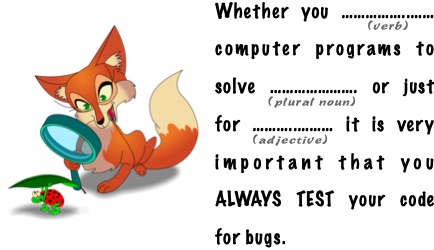
\includegraphics[width=0.75\textwidth]{images/MadLib-testing.jpg}
\end{center}
 
We need to ask the player for the following words in English:

\begin{itemize}
\item verb, for example: {\tt write}
\item plural noun, for example: {\tt problems}
\item adjective, for example: {\tt fun}
\end{itemize}

So for these examples, our program returns:

{\tt Whether you write\\ computer programs to\\ solve problems or just\\ for fun, it is very important that you\\ ALWAYS TEST your code for bugs. 
 }

Try other inputs and try to come up with a funny phrase.


\begin{domainTILEd}
This TILE contains the message that testing is important.
\end{domainTILEd}

\item Suppose you need to test a program that takes two floats as input and produces a boolean as the result. A test case for this program consists of:
   
   \begin{itemize}
      \item an identifier
      \item two float type inputs 
      \item an expected bool type output
      \item the result of the test test: ''PASS'' or ''FAIL''
  \end{itemize}
  
Write a Python program that asks the user for the following data:
  
  \begin{itemize}
      \item an integer ({\tt i})
      \item two floats ({\tt f1} and {\tt f2})
      \item a bool ({\tt out})
      \item a String ({\tt result})
  \end{itemize}
  
Your program must generate a string that uses the requested data and that describes the test case. For example, if:
  
 {\tt i = 2
 
 f1 = 123.456
 
 f2 = 12345.67
 
 out = True
 
 result = PASS}

your program should produce:

\verb|TEST_ID_002 --- inputs: 1.23e+02, 1.23e+04 --- output: True --- result: PASS|

The first part of the string is used to classify test cases: it always has to start with \verb|'test_ID_'| followed by an identifier of maximum 3 digits. If {\tt i} has fewer digits then it must be filled with leading zeros.

Floats must be presented in scientific format.

You have to do 2 different implementations of your program. One using the String module operator \% to format, and another with the \verb|str.format()|.

\begin{howTILEd}
This exercise is about creating strings that have certain patterns using string manipulation. It used to be about file names, it was TILEd by making it about test cases and their components.
\end{howTILEd}


\item Implement a program that reads three integer values: day, month, and year of a person's birth. Using this data, the program should show a four-digit PIN associated with the date of birth. The PIN is calculated as:

\begin{enumerate}
    \item p1 = (d1 + d2)\% 10.
    \item p2 = (m1 + m2)\% 10.
    \item p3 = (y1 + y4)\% 10.
    \item p4 = (y2 + y3)\% 10.
\end{enumerate}
For example, if the date entered is 29 9 1975, the PIN would be 1 9 6 6:
\begin{enumerate}
    \item p1 = (2 + 9)\% 10 = 1.
    \item p2 = (0 + 9)\% 10 = 9.
    \item p3 = (1 + 5)\% 10 = 6.
    \item p4 = (9 + 7)\% 10 = 6.
\end{enumerate}

\begin{Verbatim}[frame=single, label={\em example test execution of the program}]
>>> %Run 
  Enter your day of birth: 29
  Enter your month of birth: 9
  Enter your year of birth: 1975
  Your PIN is 1 9 6 6 
\end{Verbatim}


\begin{tabular}{|l|l|l|l|l|}
\hline
\multirow{2}{*}{test case ID} & \multicolumn{3}{l|}{inputs} & \multirow{2}{*}{expected output (PIN)}   \\ \cline{2-4} 
             & day & month & year &  \\
\hline\hline
1 & 10 & 12 & 1522 & 1 3 7 2  \\
2 & 1 & 1 & 1 & 1 1 1 0 \\
3 & 27  & 3  & 1978 & 9 3 9 6 \\
4 & 55  & 28  & 300 & 0 0 0 3 \\
5 & 356 & 903 & 1568 & 1 3 9 1 \\
\hline
\end{tabular}

Look at test cases 4 and 5. Are they valid? Inputs 55 and 356 are not valid numbers for a day of birth. However, our program works and calculates a PIN. Python does not know what birthdays are and when they are valid. For Python the 3 inputs are simply whole numbers. If we want our program not to calculate a PIN when the date is not valid, then we should add conditions that verify the inputs. We will see how we can do it in the next thematic unit with decision statements like \verb+if - then - else+.

\begin{howTILEd}
A table with test cases was added and the student were made aware of the test cases that not really contained valid dates but still calculated a PIN number.
\end{howTILEd}


\item  Write a Python program that asks the user for something that seems important to him and returns the following ASCII art (\url{https://en.wikipedia.org/wiki/ASCII\_art}):

\begin{Verbatim}[frame=none]
 >>> %Run
 Name something important: Testing your own code

                \|||||/               
                ( O O )                
|---------ooO-----(_)-----------------|
|                                     |
| Testing your own code is important! |
|                                     |
|-------------------------Ooo---------|
                |_||_|                 
                ||  ||                 
               ooO  Ooo                
\end{Verbatim}

You can use the \verb|len()| Python function that returns the length of a String (for example, \verb|len("Python")| returns 6). 
  
Your program must work with any length name:

\begin{Verbatim}[frame=none]
 >>> %Run
 Name something important: Testing your program with all kinds of different input values

                                    \|||||/                                   
                                    ( O O )                                    
|-----------------------------ooO-----(_)-------------------------------------|
|                                                                             |
| Testing your program with all kinds of different input values is important! |
|                                                                             |
|---------------------------------------------Ooo-----------------------------|
                                    |_||_|                                     
                                    ||  ||                                     
                                   ooO  Ooo                                                                               
\end{Verbatim}

\begin{howTILEd}
This TILE contains the message that testing is important.
\end{howTILEd}


\item We want to format a shopping list for a party with the following products: beer, wine and chips. You have to ask the user for the prices of the 3 products (we assume that they are always $< 10$ euros), and the quantities they want to buy (we assume that they are always $<100$ units). The program must return the purchase itemized as follows:

\begin{Verbatim}[frame=single, label={\em example test execution of the program}]
>>> %Run 
  Beer price? 9.99
  Wine price? 1.05
  Chips price? 4
  How much beer? 99
  How much wine? 23
  How many bags of chips? 1
  --------------------------
  Total purchase
  --------------------------
  Beer           99   989.01
  Wine           23    24.15
  Chips          01     4.00
                       -----
              Total  1017.16
\end{Verbatim}


You have to do 2 different implementations of your program. One using the String module operator \% to format, and another with the \verb|str.format()|. Test your program with different prices ($<10$ euros) and quantities ($<100$ units) to test that the layout is always aligned.

\begin{howTILEd}
We added one sentence explicitly asking the students to test with some values and check the output.
\end{howTILEd}




\end{enumerate}


\hypertarget{boletin3}{%
\section{Conditionals: If-then-else}\label{section.if-then-else}}

\begin{enumerate}
%\setlength{\itemindent}{1.5cm}

\item Write a program that converts a number of seconds into days, hours, minutes, and seconds. The output of your program must have the layout as in the following examples:

\begin{small}
\begin{Verbatim}[frame=single, label={\em examples of test executions}]
>>> %Run 
  Enter a number of seconds: 184
  The equivalent duration is 0:00:03:04.
>>> %Run 
  Enter a number of seconds: 6756456
  The equivalent duration is 78:04:47:36.
>>> %Run 
  Enter a number of seconds: -2
  Only positive values
\end{Verbatim}
\end{small}
To test your program, think about the inputs you want to use for the test cases and check the output by using the following converter:

{\small \url{https://www.convert-me.com/en/convert/time/second/second-to-dhms.html}}

In this way we are using another program to test the output of our program. The other program tells us what the expected results are, to compare them with the actual results of the program we are testing. In testing it is called an {\em oracle}.

The term oracle derives from the Latin oraculum that means the answer of a divinity to the questions that are posed to them. In testing, the question we ask is: what are the expected outputs of this program?
%
A test oracle can be an existing system, a user manual, the exercise description, or the specialist knowledge of the programmer, but it should not be the code.

\begin{howTILEd}
We invite the student to test their program more and compare their outcomes with a parallel oracle that they can find on the web. Moreover, we explain the terminology oracle.
\end{howTILEd}


\item A bakery sells slices of bread for 3.49 euros each. A day old bread gets a discount of 60 percent.
%
Write a program that asks the user for the number of day old loaves of bread they want to buy. Then your program should show the price of bread, the discount for being a day old and the total price. Each one of these amounts must be shown on their own line with a suitable label. Every values should be displayed using two decimal places, and decimal points in
all numbers should line up when the user enters reasonable values.

You have to test your program to see if it works well.

\begin{small}
\begin{Verbatim}[frame=single, label={\em examples of test executions}]
>>> %Run 
  Enter the number of day old loaves: 45
  -------------------------
  Regular price:     157.05
  Discount:           94.23
  -------------------------
  Total:              62.82

>>> %Run 
  Enter the number of day old loaves: 0
  -------------------------
  Regular price:       0.00
  Discount:            0.00
  -------------------------
  Total:               0.00

>>> %Run 
  Enter the number of day old loaves: -4
  You cannot buy negative amounts of bread
\end{Verbatim}
\end{small}

\begin{howTILEd}
Insist that the students test their programs by giving them example test executions.
\end{howTILEd}


\item Write a Python program that asks the user for a word $p$ and
it returns in the output another word in which the first and last characters of $p$ have been exchanged. Use the chain cutter operator. Run the following tests to test the operation of your program:

\begin{tabular}{|l|l|l|}
\hline
test case ID & input & expected output  \\ 
\hline\hline
1 & \verb+""+ & \verb+""+ \\
2 & \verb+"a"+ & \verb+"a"+\\
3 & \verb+"ab"+ & \verb+"ba"+\\
4 & \verb+"ab ba"+ & \verb+"ab ba"+\\
\hline
\end{tabular}


\begin{howTILEd}
Insist that the students test their programs by giving them a table of test cases.
\end{howTILEd}

\item Write a program that reads an integer number and tells whether it is odd or even. Run the following examples to test that your program gives the same outputs:

\begin{small}
\begin{Verbatim}[frame=single, label={\em examples of test executions}]
>>> %Run 
  Enter an integer number: 1
  The number 1 is odd
>>> %Run 
  Enter an integer number: 0
  The number 0 is even
>>> %Run 
  Enter an integer number:111
  The number 1 is odd
>>> %Run 
  Enter an integer number: 23
  The number 23 is odd
>>> %Run 
  Enter an integer number: -34
  The number 0 is even
>>> %Run 
  Enter an integer number: -11
  The number -11 is odd
\end{Verbatim}
\end{small}

\begin{howTILEd}
Insist that the students test their programs by giving them example test executions.
\end{howTILEd}

\item Implement a program that reads three values and displays on the screen the maximum and the minimum. Run the following examples to test that your program gives the same outputs:

\begin{small}
\begin{Verbatim}[frame=single, label={\em examples of test executions}]
>>> %Run 
  Enter the first value: 3
  Enter the second value: 6
  Enter the third value: 8
  The maximum is 8 and the minimum is 3
>>> %Run 
  Enter the first value: -4
  Enter the second value: 6
  Enter the third value: 12
  The maximum is 6 and the minimum is -4
>>> %Run
  Enter the first value: 4.567
  Enter the second value: 9
  Enter the third value: 12.9
  The maximum is 9 and the minimum is 12.9
>>> %Run 
  Enter the first value: a
  Enter the second value: c
  Enter the third value: h
  The maximum is h and the minimum is a
>>> %Run 
  Enter the first value: hello
  Enter the second value: hola
  Enter the third value: bonjour
  The maximum is hola and the minimum is bonjour
>>> %Run 
  Enter the first value: 4
  Enter the second value: oh!
  Enter the third value: 4.89
  The maximum is oh! and the minimum is 4
\end{Verbatim}
\end{small}

\begin{howTILEd}
Insist that the students test their programs by giving them example test executions. The values used in the example test executions will make then aware that the program was not only for numerical values but for any value.
\end{howTILEd}


\item Implement a program that reads an integer corresponding to a month of the year and displays the name of the corresponding month. If the entered number does not belong to the range [1, 12], an error message will be displayed.

\begin{small}
\begin{Verbatim}[frame=single, label={\em examples of test executions}]
>>> %Run 
  Enter the number of the month: 5
  May
>>> %Run 
  Enter the number of the month: 12
  December
>>> %Run 
  Enter the number of the month: 13
  Error: enter a number between 1 y 12
>>> %Run 
  Enter the number of the month: -3
  Error: enter a number between 1 and 12
>>> %Run 
  Enter the number of the month: 0
  Error: enter a number between 1 and 12
\end{Verbatim}
\end{small}

\begin{howTILEd}
Insist that the students test their programs by giving them example test executions.
\end{howTILEd}

\item Implement a program that reads two integer numbers and says if their product is positive, negative, or zero \textbf{without} doing the calculation.

Run the following combinations of examples to test that your program produces the same outputs: 
\begin{itemize}
\item the first number is 0, 
\item the second number is 0, 
\item both numbers are 0, 
\item both numbers are positive, 
\item both numbers are negative, 
\item the first number is negative and the second is positive, 
\item the first number is positive and the second is negative.
\end{itemize}

\begin{small}
\begin{Verbatim}[frame=single, label={\em examples of test executions}]
>>> %Run
  Enter the first integer number: 0
  Enter the second integer number: -1
  The product is zero
>>> %Run 
  Enter the first integer number: 5
  Enter the second integer number: 0
  The product is zero
>>> %Run 
  Enter the first integer number: 0
  Enter the second integer number: 0
  The product is zero
>>> %Run 
  Enter the first integer number: 2
  Enter the second integer number: 7
  The product is positive
>>> %Run 
  Enter the first integer number: -4
  Enter the second integer number: -7
  The product is positive
>>> %Run 
  Enter the first integer number: -8
  Enter the second integer number: 3
  The product is negative
>>> %Run 
  Enter the first integer number: 10
  Enter the second integer number: -6
  The product is negative
\end{Verbatim}
\end{small}

\begin{howTILEd}
Insist that the students test their programs by giving them example test executions. Also pointing out that this way we try out all possible combinations to test.
\end{howTILEd}


\item Write a program that reads an age, and finds out if someone is in their babyhood, childhood, adolescence, initial adulthood, mature adulthood, or old age. Use the following approximate definitions:

\begin{itemize}
\item Babyhood starts at birth and ends at 2 years of age.
\item Childhood ranges from 2 to 12 years of age
\itemcorresponde The adolescence corresponds to the age ranging from 12 to 20 years.
\item Initial adulthood ranges from 20 to 40 years of age.
\item Mature adulthood begins at age 40 and ends at age 60.
\item Old age goes from 60 years on wards.
\end{itemize}

Run tests and ensure that each of the possible outputs has occurred at least once.

\begin{howTILEd}
Add minimal line saying the should test such that each possible output has occurred.
\end{howTILEd}


\item The density (d) of a substance is defined as the amount of mass (m) it has per volume unit (v). Then:

\[d = \frac{m}{v} \;\;\leftrightarrow\;\; m = d \times v \;\;\leftrightarrow\;\; v = \frac{m}{d} 
\]

Write a program that asks the user what he wants to calculate (density, mass or volume), then asks for the necessary data and at the end prints the result on the screen.

Run the following examples to test that your program gives the same outputs.

\begin{small}
\begin{Verbatim}[frame=single, label={\em examples of test executions}]
>>> %Run 
  What do you want to calculate? (d, m, v):d
  Mass: 45
  Volume: 67
  The density is:  0.6716417910447762
>>> %Run 
  What do you want to calculate? (d, m, v):d
  Mass: 45
  Volume: 0
  Cannot be calculated
 >>> %Run 
  What do you want to calculate? (d, m, v):m
  Densidad: 34
  Volume: 67
  The mass is:  2278
>>> %Run 
  What do you want to calculate? (d, m, v):m
  Densidad: 0
  Volume: 25
  The mass is:  0
>>> %Run 
  What do you want to calculate? (d, m, v):v
  Densidad: 56
  Mass: 900
  The volume is: 16.071428571428573
>>> %Run 
  What do you want to calculate? (d, m, v):v
  Densidad: 0
  Mass: 568
  The mass is
>>> %Run 
  What do you want to calculate? (d, m, v): z
  Enter only d, m or v
\end{Verbatim}
\end{small}

\begin{howTILEd}
Insist that the students test their programs by giving them example test executions. 
\end{howTILEd}


\item Implement a program that asks the user for a relational operator (\verb|<, <=, >, >=, ==, !=|) and 2 values. Your program has to display on screen the result (\verb+True+ or \verb+False+) of the given operation applied to the two values.

You can design the layout of the input and output of your program as you want. Run the following test cases to test the operation of your program:

\begin{tabular}{|l|l|l|l|l|}
\hline
\multirow{2}{*}{test case ID} & \multicolumn{3}{l|}{inputs} & \multirow{2}{*}{expected output}   \\ \cline{2-4} 
             & operator & value1 & value2 &  \\
\hline\hline
1 & \verb+<+ & 12 & 4 & \verb+False+ \\
2 & \verb+>+ & 100 & 40 & \verb+True+ \\
3 & \verb+==+ & \verb+"Hello!"+ & 40 & \verb+False+ \\
4 & \verb+!=+ & 100 & \verb+"Python"+ & \verb+True+ \\
5 & \verb+>=+ & 98.67 & 0.45 & \verb+True+ \\
6 & \verb+<=+ & -100 & 40 & \verb+True+ \\
7 & \verb+<+ & 24 & \verb+"24K"+ & \verb+True+ \\
8 & \verb+>=+ & \verb+"email"+ & \verb+"correo"+ & \verb+True+ \\
\hline
\end{tabular}

\begin{howTILEd}
Insist that the students test their programs by giving them example test cases in a table. Again the chosen values will make them aware that this is not only for numerical values.
\end{howTILEd}



\item Implement a program that reads three integer numbers:
\verb+a+, \verb+b+ and \verb+c+. The program must indicate whether the numbers can represent the sides of a triangle. For this, each value must be less than the sum of the other two. If so, the program must indicate if it is a:

\begin{itemize}
\item scalene triangle (if all three sides are different), 
\item equilateral triangle (if all three sides are equal), or
\item isosceles triangle (two equal sides and one different).
\end{itemize}

This triangle challenge is well known. It was proposed by
Jerry Weinberg\footnote{\url{https://en.wikipedia.org/wiki/Gerald_Weinberg}}, a famous computer scientist, and described by Glenford Myers, who wrote the first book on software testing, the classic The Art of Software Testing\footnote{\url{https://onlinelibrary.wiley.com/doi/book/10.1002/9781119202486}}.

Test your program with the set of test cases proposed below:


\begin{tabular}{|l|l|l|l|l|}
\hline
\multirow{2}{*}{test case ID} & \multicolumn{3}{l|}{inputs} & \multirow{2}{*}{expected output}   \\ \cline{2-4} 
             & \verb+a+ & \verb+b+ & \verb+c+ &  \\
\hline\hline
1  & 1 & 50 & 50 & Isosceles \\
2           & 2          & 50          & 50          & Isosceles          \\
3           & 99         & 50          & 50          & Isosceles          \\
4           & 100        & 50          & 50          & Not a Traingle     \\
5           & 50         & 50          & 50          & Equilateral        \\
6           & 50         & 1           & 50          & Isosceles          \\
7           & 50         & 2           & 50          & Isosceles          \\
8           & 50         & 99          & 50          & Isosceles          \\
9           & 50         & 100         & 50          & Not a Triangle     \\
10          & 50         & 50          & 1           & Isosceles          \\
11          & 50         & 50          & 2           & Isosceles          \\
12          & 50         & 50          & 99          & Isosceles          \\
13          & 50         & 50          & 100         & Not a Triangle   \\
\hline
\end{tabular}

\begin{howTILEd}
Insist that the students test their programs by giving them test cases. Also include a bit of anecdotal history on the triangle program and first book on software testing.
\end{howTILEd}


\item Read an amount of euros and display the minimum breakdown in bills and coins for that amount on the screen. This means that the minimum number of bills/coins must be returned. We assume that there are 500, 200, 100, 50, 20, 10 and 5 bills, and 2 and 1 coins.

Write a version of this program that shows the breakdown on the screen mentioning only the bills and coins we need.

\begin{small}
\begin{Verbatim}[frame=single, label={\em examples of test executions}]
>>> %Run 
  Enter an amount of euros: 434
  2 bills of 200
  1 bill of 20
  1 bill of 10
  2 coins of 2
>>> %Run 
  Enter an amount of euros: 0
  There are no bills or coins
>>> %Run 
  Enter an amount of euros: -35
  There are no bills or coins
>>> %Run 
  Enter an amount of euros: 1
  1 coin of 1
>>> %Run 
  Enter an amount of euros: 5
  1 bill of 5
\end{Verbatim}
\end{small}

What other tests could you run to ensure that your program has the desired behaviour? Have you tried, for example, entering different amounts that return all the bills and coins at least once? For example:

\begin{itemize}
    \item for quantity 2, a coin of 2 must be returned
    \item for quantity 10, a bill of 10 must be returned 
    \item for quantity 20, \dots
    \item etc.
\end{itemize}


Have you tried, for example, entering different amounts to test whether your program returns the minimum number of correct combinations of bills and coins? For example:

\begin{itemize}
    \item for quantity 6, a bill of 5 and a coin of 1 must be returned (and not for example 3 coins of 2)
     \item for quantity 12, a bill of 10 and a coin of 2 must be returned (and not for example two bills of 5 and two coins of 1)
     \item for quantity 24, \dots
     \item etc.
\end{itemize}


\begin{howTILEd}
Insisting that the students test their programs and think about all possible combinations.
\end{howTILEd}


\item Implement a program that reads the duration in seconds of a phone call and determines the total amount to be paid. The business rule is: {\em if the call lasts less than 1 minute it costs 10 cents, and each additional minute from the first one costs 5 cents}. 

For example, if the call lasts 35 seconds, the cost will be 10 cents. If it lasts 3 minutes and 40 seconds (that is, the user will enter the value 220), it will cost 20 cents: 10 cents for the first minute plus 5 cents for the next 2 minutes. The remaining 40 seconds are free.

\begin{small}
\begin{Verbatim}[frame=single, label={\em examples of test executions}]
>>> %Run 
  Enter the number of seconds the call has lasted: 0
  The call has a cost of 0 cents
>>> %Run 
  Enter the number of seconds the call has lasted: 5
  The call has a cost of 10 cents
>>> %Run 
  Enter the number of seconds the call has lasted: 59
  The call has a cost of 10 cents
>>> %Run 
  Enter the number of seconds the call has lasted: 125
  The call has a cost of 15 cents
>>> %Run 
  Enter the number of seconds the call has lasted: 200
  The call has a cost of 20 cents
>>> %Run 
  Enter the number of seconds the call has lasted: -5
  Please enter a correct value
\end{Verbatim}
\end{small}

What other tests have you run to ensure that your program has the desired behaviour?


\begin{howTILEd}
Insist that the students test their programs by giving them example test executions and ask them to think about more tests.
\end{howTILEd}

\item The water company is implementing a new billing system. For each house, the invoice is made as follows: 
\begin{enumerate}
\item The first 50 litres are free.
\item Between 50 and 200 litres, each litre is charged at 0.10 euros.
\item From 200 litres on, each litre is charged at 0.30 euros.
\item The minimum fee is 6 euros, that is, if the amount to pay is less than 6 euros, then the payment will be 6 euros.
\end{enumerate}
Write a program that calculates the water consumption of a family in a month given the number of litres used.

\begin{small}
\begin{Verbatim}[frame=single, label={\em examples of test executions}]
>>> %Run 
  Enter the litres of water used: 0
  The expense is 6.00€
>>> %Run 
  Enter the litres of water used: -500
  Please enter a correct value
>>> %Run 
  Enter the litres of water used: 300
  The expense is 90.00€
>>> %Run 
  Enter the litres of water used: 55
  The expense is 6.00€
\end{Verbatim}
\end{small}

\begin{howTILEd}
Insist that the students test their programs by giving them example test executions. 
\end{howTILEd}


\item A book store gives discounts to its customers depending on whether the customer has the membership card and the price of the purchase made.

\begin{itemize}
\item below 10 euros no discount is applied to anyone
\item between 10 and 20 euros, a 5\% discount is applied when the customer has the membership card
\item above 20 euros, a discount of 12\% is applied when the customer has the membership card, and 6\% where there is no card.
\end{itemize}

Write a program that asks the user by keyboard how much the purchase is, and whether the customer is a member or not. Depending on these input data, the program has to show on the screen how much the customer has to pay for the purchase.

Run the following test cases to ensure that the program works correctly:

\begin{tabular}{|l|l|l|}
\hline
ID & abstract test case & expected result\\
\hline\hline
1 & member with purchase under 10 euros & discount 0\%\\
2 & non-member with purchase below 10 euros & discount 0\%\\
3 & member with purchase between 10 and 20 euros & discount 5\%\\
4 & non-member with purchase between 10 and 20 euros & discount 0\%\\
5 & member with purchase over 20 euros & discount 12\%\\
6 & non-member with purchase over 20 euros & discount 6\%\\
\hline
\end{tabular}

We call these test cases {\em abstract} because, in order to execute them, we first have to think of concrete values that meet the conditions of the test case.

\begin{howTILEd}
Insist that the students test their programs by giving them example test cases in a table. Also we introduce the concept of abstract vs concrete test cases. 
\end{howTILEd}

\item Write a program that determines if an athlete is selected to run a marathon. To be selected, the qualifying times are:

\begin{itemize}
    \item 150 minutes for men under 40
    \item 175 minutes for men over 40
    \item 180 minutes for women
\end{itemize}

The data to be entered are: sex (possible values: M, F), age and time. It is necessary to verify if the entered data have suitable values, and if not, indicate it and stop the program. When the data is correct, the program will display the message ''Selected'' or ''Not selected''.

\begin{small}
\begin{Verbatim}[frame=single, label={\em examples of test executions}]
>>> %Run 
  Sex M/F: Y
  Enter only the letters M or F
>>> %Run 
  Sex M/F: F
  Age: -4
  Enter a correct age
>>> %Run 
  Sex M/F: M
  Age: 14
  Time: -400
  Enter a correct time
>>> %Run 
  Sex M/F: M
  Age: 14
  Time: 300
  Not selected
>>> %Run 
  Sex M/F: M
  Age: 50
  Time: 170
  Selected
\end{Verbatim}
\end{small}

What other tests do you have to run to ensure that you have tried all the possible combinations? (HINT: in the tests above we have never tested the outputs when the sex is \verb+F+)


\begin{howTILEd}
Insist that the students test their programs by giving them example test executions.  Add a comment on tests that might be missing and that they have to think about.
\end{howTILEd}


\item Write a Python program that determines the cost of a car insurance depending on:
the age of the person to be insured, 
and the number of years this person has a driver's license, and the number of accidents the person has been involved in. The program will ask for these data (in that order) to be entered by keyboard, and will return the amount of insurance if possible, taking into account that:
\begin{enumerate}[a)]
    \item The customer must be over 18 years of age to be able to insure.
    \item The base amount is 300 euros.
    \item 200 euros are added if the license is less than 3 years old, 150 euros are added between 3 (inclusive) and 5 years (not inclusive), or 100 euros are added between 5 and 10 years (both inclusive).
    \item 200 euros are added if the age of the customer is under 25 years old.
    \item There is an additional charge depending on the number of accidents:
\end{enumerate}

\begin{table}[htbp]
\begin{center}
\begin{tabular}{|l|l|}
\hline
Accidents & Charge (euros) \\
\hline \hline
1 & 50 \\ \hline
2 & 125 \\ \hline
3 & 225 \\ \hline
4 & 375 \\ \hline
5 & 575 \\ \hline
6 or more & Not insured \\ \hline
\end{tabular}
\label{tabla:sencilla}
\end{center}
\end{table}

\begin{small}

\begin{Verbatim}[frame=single, label={\em examples of test executions}]
>>> %Run 
  Age: 10
  You have to be 18 or over to have car insurance.
>>> %Run 
  Age: 18
  Years with license: 0
  Number of accidents: 0
  The amount of the insurance is:  700 €
>>> %Run 
  Age: 30
  Years with license: 3
  Number of accidents: 1
  The amount of the insurance is:  500 €
>>> %Run 
  Age: 20
  Years with license: -4
  Enter an appropriate number of years
>>> %Run 
  Age: 20
  Years with license: 4
  Number of accidents: -7
  Enter a positive number
\end{Verbatim}
\end{small}

What other tests have you run to ensure that your program has the desired behaviour?

Have you tried ages that lead to different behaviours? Try with the test cases ({\tt age $\le$ 25}), ({\tt age $\ge$ 25}) and also when the age is exactly 25, a value located between the two behaviour intervals.

Have you tested your program for all possible ranges of years that the user can have the license? For example, the test cases for the years intervals {\tt [0, 3[}, {\tt [3, 5[} and {\tt [5, 10]}.

Have you tested your program with all possible values for the number of accidents?

And how about different combinations of the cases mentioned above?

\begin{howTILEd}
Insist that the students test their programs by giving them example test executions. Moreover, guide them through a thinking process of what else needs to be tested.
\end{howTILEd}


\item An expert system is a type of artificial intelligence program that uses a knowledge base and a set of rules to perform a task that a human expert could do. They help self-diagnose a problem by answering a series of questions. For example, many hardware and software companies offer online troubleshooting tools to help people solve simple technical problems before calling a human.

Create a program that guides the user through the process of figuring out the type of fruit on hand. Use the following decision tree to build the system: 

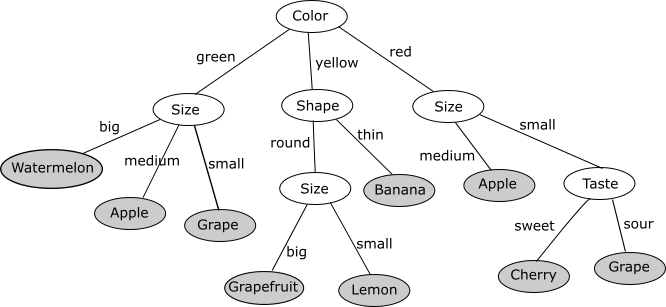
\includegraphics[width=0.85\textwidth]{images/tree.png}

\begin{small}
\begin{Verbatim}[frame=single, label={\em examples of test executions}]
>>> %Run 
  Color (green/yellow/red): green
  Size (big/medium/small): big
  Watermelon
>>> %Run 
  Color (green/yellow/red): yellow
  Shape (round/thin): round
  Size (big/small): big
  Grapefruit
\end{Verbatim}
\end{small}
To test your program very well you should have a test case for each of the 9 fruits on the tree.

\begin{howTILEd}
Insist that the students test their programs by giving them example test executions and ask them to add more tests such that each possible inputs occurs once. 
\end{howTILEd}


\item You want to create a Python program to calculate different areas. To do this, the program will present the option of
area to be calculated. The possible options are:
\begin{enumerate}
\item Calculation of the area of a square: area = side**2
\item Calculation of the area of a triangle: area = (base * height)/2
\item Calculation of the area of a rectangle: area = side1 * side2
\end{enumerate}
Once the option has been chosen, the necessary data will be requested and the corresponding result will be presented.
In the event that the specified option was not
correct, the phrase ''incorrect value" would be displayed on the screen.

\begin{small}
\begin{Verbatim}[frame=single, label={\em examples of test executions}]
>>> %Run 
  Area (square/triangle/rectangle): square
  Side: 3.56
  The area of the square is: 12.6736
>>> %Run 
  Area (square/triangle/rectangle): triangle
  Base: 18
  Height: 4
  The area of the triangle is: 36.0
>>> %Run 
  Area (square/triangle/rectangle): rectangle
  Side 1: 4.67
  Side 2: 9
  The area of the rectangle is: 42.03
>>> %Run 
  Area (square/triangle/rectangle): hello
  Wrong value
>>> %Run 
  Area (square/triangle/rectangle): square
  Side: -4
  Wrong value
\end{Verbatim}
\end{small}

\begin{howTILEd}
Insist that the students test their programs by giving them example test executions. 
\end{howTILEd}



\item Write a Python program to determine the quadrant of the Cartesian plane given the (x, y) coordinates of a point.

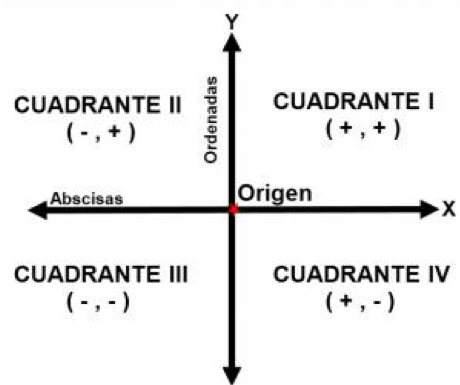
\includegraphics[width=0.4\textwidth]{images/cuadrant.png}

To test this program try to execute a test case for each one of the possible 9 outputs (i.e. the 4 different pieces of axis, the origin and the 4 different quadrants).

\begin{howTILEd}
Insist that the students test their programs by giving them hints on what to test to get all possible outputs.
\end{howTILEd}





\item Implement a Python program that asks the user for four inputs:
a serial number, a day, a month, and a year of production date.
First your program has to verify that the given day, month and year correspond to a correct date. If not, your program will notify that on the screen and it will stop. You can finish a program with the instruction \verb|exit()|.

If the date is correct, then you have to check if the serial number corresponds to the production date and print the result on the screen.

The serial number has to be 8 numbers long (remember the use of the \verb|len()| function), any number with another length is wrong.

Then we should check whether the serial number is correct and inform the user.
A serial number is correct when:

\begin{enumerate}
\item The first 4 digits of the number (n1, n2, n3 and n4) meet the following properties:

\begin{enumerate}
    \item n1 = (d1 + d2)\% 10.
    \item n2 = (m1 + m2)\% 10.
    \item n3 = (y1 + y4)\% 10.
    \item n4 = (y2 + y3)\% 10.
\end{enumerate}

\item The sum of the last 4 digits of the number (n5, n6, n7 and n8) must be less than 25.
\end{enumerate}

What tests have you run to ensure that your program has the desired behaviour? Note that dates can be incorrect in many ways, make sure your program detects them all and stops when you enter:

\begin{itemize}
    \item day that is $\leq 0$
    \item month that is $\leq 0$
    \item year that is $< 0$ (do we accept the year 0?)
    \item days $>=31$ for months that only have 30 days
    \item days $>=32$ for months that only have 31 days
    \item 29th of February when it is not a leap year
\end{itemize}

Then for correct dates, calculate some serial numbers by hand such that you can test the output of your program.

\begin{howTILEd}
Insist that the students test their programs by giving them hints on what to test.
\end{howTILEd}

\end{enumerate}


\hypertarget{boletin4}{%
\section{Loops}\label{section.loops}}

\begin{enumerate}
%\setlength{\itemindent}{1.5cm}

\item Write a program to calculate the sum of the integers between $N$ and $M$, where $N$ and $M$ are values entered by the user.
%
\verb+result+ = $\sum_{n = N}^{M} n$

\begin{Verbatim}[frame=single, label={\em examples of test executions}]
>>> %Run 
  Enter a number: 0
  Enter a number: 3
  The sum from 0 to 3 is:  6
>>> %Run 
  Enter a number: -5
  Enter a number: 3
  The sum from -5 to 3 is: -9
>>> %Run 
  Enter a number: -8
  Enter a number: 8
  The sum from -8 to 8 is:  0
>>> %Run 
  Enter a number: 4
  Enter a number: 4
  The sum from 4 to 4 is:  4
\end{Verbatim}


\begin{howTILEd}
Insist that the students test their programs by giving them example test executions. 
\end{howTILEd}



\item Implement a program to read 10 positive numbers and independently calculate the sum of the odd and even numbers. If a negative number is entered, the program will display an error message and ask for the number again.

\begin{Verbatim}[frame=single, label={\em examples of test executions}]
>>> %Run 
  Enter a number: 4
  Enter a number: 5
  Enter a number: 6
  Enter a number: 7
  Enter a number: 8
  Enter a number: 9
  Enter a number: 12
  Enter a number: -4
  Please enter only positive numbers
  Enter a number: 0
  Enter a number: 3
  Enter a number: 209
  Sum of the even numbers:  30
  Sum of the odd numbers:  233
>>> %Run
  Enter a number: -4
  Please enter only positive numbers
  Enter a number: -0
  Enter a number: 4
  Enter a number: 4
  Enter a number: 5
  Enter a number: 5
  Enter a number: 6
  Enter a number: 6
  Enter a number: 7
  Enter a number: 7
  Enter a number: 8
  Sum of the even numbers:  28
  Sum of the odd numbers:  24
>>> %Run 
  Enter a number: 2
  Enter a number: 4
  Enter a number: 6
  Enter a number: 8
  Enter a number: 0
  Enter a number: 16
  Enter a number: 18
  Enter a number: 20
  Enter a number: 36
  Enter a number: 90
  Sum of the even numbers:  200
  Sum of the odd numbers:  0
\end{Verbatim}

\begin{howTILEd}
Insist that the students test their programs by giving them example test executions. 
\end{howTILEd}



\item Implement a program that reads 12 real numbers and calculates the mean of the positive and negative numbers. Afterwards, the result must be displayed to a maximum of 4 decimal places. Run the following test cases to test your program:

\begin{tabular}{|l|l|l|l|}
\hline
test  & \multirow{3}{*}{inputs} & \multicolumn{2}{l|}{expected outputs}  \\ \cline{3-4} 
case     &  & mean of & mean of     \\
ID       &  & positives & negatives    \\
\hline\hline
1 & 1, 2, 3, 4, 5, 6, 7, 8, 9, 10, 11, 12  &  6.5 & 0  \\
2 & -1, -2, -3, -4, -5, -6, -7, -8, -9, -10, -11, -12  &  0 & -6.5  \\
3 & 0, 0, 0, 0, 0, 0, 0, 0, 0, 0, 0, 0 & 0 & 0 \\
4 & 12.4, 21.005, -3.67, 4.43, 5.56, 4.2, 7, 8.3, -91.3, -1.0, 32.4, 12.1 & 11.9327 & -31.99\\
\hline
\end{tabular}




\begin{howTILEd}
Insist that the students test their programs by giving them example test cases in a table. Series with only positive numbers, series with only negative numbers, all zeros, and mix of positive/negative.
\end{howTILEd}





\item Write a program that receives an integer $N$ and generates all the multiples of 7 between 1 and $N$. Run the following test cases to test your program:

\begin{tabular}{|l|l|l|l|}
\hline
test case ID  & inputs & expected outputs  \\ 
\hline\hline
1 & 0 & there are no multiples of 7\\
2 & 3 & there are no multiples of 7\\
3 & -5 & there are no multiples of 7\\
4 & -15 & -7, -14\\
5 & 18 & 7, 14\\
6 & 57 & 7, 14, 21, 28, 35, 42, 49, 56\\
\hline
\end{tabular}

\begin{howTILEd}
Insist that the students test their programs by giving them example test cases in a table. Again the chosen values will make them aware that there program should also work for negative numbers.
\end{howTILEd}


\item Modify the previous program so that it displays only those multiples of 7 between 1 and $N$ that are not divisible by 3. Execute the following test cases to test your program:

\begin{tabular}{|l|l|l|l|}
\hline
test case ID  & inputs & expected outputs  \\ 
\hline\hline
1 & 0 & there are no multiples of 7\\
2 & 3 & there are no multiples of 7\\
3 & -5 & there are no multiples of 7\\
4 & -65 & -7, -14, -28, -35, -49, -56\\
5 & 18 & 7, 14\\
6 & 77 & 7, 14, 28, 35, 49, 56, 70, 77\\
\hline
\end{tabular}


\begin{howTILEd}
Insist that the students test their programs by giving them example test cases in a table.
\end{howTILEd}




\item We have a total of 15 test cases of a Python program. From each test we run, we take note of the number of failures that finds. So at the end we have a set of 15 natural numbers: From $n_1$ to $n_{15}$.

We are going to write a program that asks for these 15 natural numbers through the keyboard and determines:

\begin{itemize}
\item How many tests have not found any error, that is, 0.
\item How many tests have found between 1 and 3 errors.
\item How many have found more than 4 errors.
\end{itemize}

In the execution example below you can see how your program should handle negative numbers.

\begin{Verbatim}[frame=single, label={\em examples of test executions}]
>>> %Run 
  Enter the number of bugs found by test 1: 3
  Enter the number of bugs found by test 2: 4
  Enter the number of bugs found by test 3: -5
  You cannot enter negative amounts.
  Enter the number of bugs found by test 3: 5
  Enter the number of bugs found by test 4: 6 
  Enter the number of bugs found by test 5: 7
  Enter the number of bugs found by test 6: 0
  Enter the number of bugs found by test 7: 0
  Enter the number of bugs found by test 8: 1
  Enter the number of bugs found by test 9: 2
  Enter the number of bugs found by test 10: 6
  Enter the number of bugs found by test 11: 1
  Enter the number of bugs found by test 12: 2
  Enter the number of bugs found by test 13: 0
  Enter the number of bugs found by test 14: 0
  Enter the number of bugs found by test 15: 2
  Number of tests that have found 0 errors:  4
  Number of tests that have found between 1 and 3 errors:  6
  Number of tests that have found more than 4 errors:  5
\end{Verbatim} 

\begin{domainTILEd}
Categorising series of inputs, where the inputs are related to test cases. Test cases can find errors!
\end{domainTILEd}

\item Implement a program that reads 12 real numbers and calculates the maximum. Run the following test cases to test your program:

\begin{tabular}{|l|l|l|}
\hline
test ID  & inputs & expected outputs  \\ 
\hline\hline
1 & 12.2, 6.0, 3.3, 4, 5, 6.5, 7, 8, 9, 3.3, 11, 12.2  &  12.2   \\
2 & -1, -2, -3, -4, -5, -6, -7, -8, -9, -10, -11, -12  &  -1   \\
3 & 0, 0, 0, 0, 0, 0, 0, 0, 0, 0, 0, 0 & 0  \\
4 & 12.4, 21.005, -3.67, 4.43, 5.56, 4.2, 7, 8.3, -91.3, -1.0, 32.4, 12.1 & 32.4 \\
\hline
\end{tabular}

\begin{howTILEd}
Insist that the students test their programs by giving them example test cases in a table.
\end{howTILEd}




\item Write a program that reads the grades of the students of a certain
subject until the user enters the word ''exit''. The exit of your program must write at the end the number of passed, the number of failed, and the average grade. Remember that a string can be converted to a float, by calling \verb+float+. Test it:


\begin{Verbatim}[frame=single, label={\em examples of test executions}]
>>> s = "3.456"
>>> float(s)
3.456
>>> s = "-3.456"
>>> float(s)
-3.456
\end{Verbatim} 

Some examples of program executions are below. There you can see how your program should handle negative numbers.

\begin{Verbatim}[frame=single, label={\em examples of test executions}]
>>> %Run 
  Enter a grade or 'exit': 3.5
  Enter a grade or 'exit': 0
  Enter a grade or 'exit': 10
  Enter a grade or 'exit': 9.99
  Enter a grade or 'exit': 5
  Enter a grade or 'exit': 6
  Enter a grade or 'exit': 8
  Enter a grade or 'exit': exit
  Passed: 5
  Failed: 2
  Average grade: 6.07
>>> %Run 
  Enter a grade or 'exit': -4
  You cannot enter negative amounts.
  Enter a grade or 'exit': 4
  Enter a grade or 'exit': -6.4
  You cannot enter negative amounts.
  Enter a grade or 'exit': 0
  Enter a grade or 'exit': 3
  Enter a grade or 'exit': exit
  Passed: 0
  Failed: 3
  Average grade: 2.3333333333333335  
\end{Verbatim} 

\begin{howTILEd}
Insist that the students test their programs by giving them example test executions.
\end{howTILEd}




\item Write a program that reads the age (an integer) of a set of people. Data entry will end when a negative value is entered. Your program has to calculate and display on the screen:

\begin{itemize}
\item the average of the ages, 
\item the maximum and minimum age, and
\item how many of them are people of working age, that is, their age is between 18 and 65 years old
\end{itemize}

\begin{Verbatim}[frame=single, label={\em examples of test executions}]
>>> %Run 
  Enter an age:50
  Enter an age:18
  Enter an age:0
  Enter an age:-2
  Average: 22.666666666666668
  Maximum age: 50
  Minimum age: 0
  People of working age: 2
>>> %Run 
  Enter an age:12
  Enter an age:16
  Enter an age:90
  Enter an age:65
  Enter an age:18
  Enter an age:17
  Enter an age:19
  Enter an age:66
  Enter an age:64
  Enter an age:-5
  Average: 40.77777777777778
  Maximum age: 90
  Minimum age: 12
  People of working age: 4
\end{Verbatim}

\begin{howTILEd}
Insist that the students test their programs by giving them example test executions.
\end{howTILEd}



\item Write a program that finds the first value $N$ for which the sum $0 + 1 + 2 + 3 + ... + N$ exceeds a LIMIT value that is entered by keyboard.
Run the following test cases to test your program:

\begin{tabular}{|l|l|l|}
\hline
test ID  & input & expected output  \\ 
\hline\hline
1 & 0  & 1 \\
2 & 1  &  2   \\
3 & 25 & 7  \\
4 & -5 & 0 \\
5 & -450 & 0 \\
6 & 45 & 10\\
\hline
\end{tabular}


\begin{howTILEd}
Insist that the students test their programs by giving them example test cases in a table. We have explicitly added 0 and negative numbers to make sure these are tested.
\end{howTILEd}



\item A three-digit number is called an Armstrong number if the sum of the cube of its digits equals the number itself.
For example, 153 is an Armstrong number because ($1 ^ 3$) + ($5 ^ 3$) + ($3 ^ 3$) = 153. Write all Armstrong numbers between 100 and 500.

To test your program consider these numbers, which are the only Armstrong numbers:

$153=1^3+5^3+3^3$

$370=3^3+7^3+0^3$

$371=3^3+7^3+1^3$

$407=4^3+0^3+7^3$

\begin{howTILEd}
Insist that the students test their programs by giving them the expected outcome of their program.
\end{howTILEd}


\item Write a program to determine whether an integer is prime or not. A prime number is a natural number greater than 1 that has only two positive divisors: itself and 1. For example, the prime numbers less than 200 are:
2, 3, 5, 7, 11, 13, 17, 19, 23, 29, 31, 37, 41, 43, 47, 53, 59, 61, 67, 71, 73, 79, 83, 89, 97, 101, 103, 107, 109, 113, 127, 131, 137, 139, 149, 151, 157, 163, 167, 173, 179, 181, 191, 193, 197, 199. You can use them as test cases for your program. 

Remember, you should not only tests whether primes are detected correctly. You should also test other numbers and check your program says they are not prime. Also try with negative numbers.


\begin{howTILEd}
Insist that the students test their programs by giving them ideas or pointers about the test data to use.
\end{howTILEd}


\item Implement a program that, given two integers, returns if one is a divisor of the other. To do this, you must detect which is the smallest. You cannot use the division or remainder operation. In your implementation you must also take into account negative numbers and 0 (all numbers are divisors of 0).

For your program, perhaps the \pythoninline{abs()} function from the Python standard library is useful. The \pythoninline{abs()} function returns the absolute value of the given number. The absolute value of a number is the value regardless of its sign. Therefore, the absolute of 10 is 10, and hte absolute of -10 is also 10.

Test your program with the following outputs:

\begin{Verbatim}[frame=single, label={\em examples of test executions}]
>>> %Run 
  Enter an integer number: 0
  Enter another integer number: 0
  There are no divisors of 0
>>> %Run 
  Enter an integer number: 0
  Enter another integer number: 2
  2 is a divisor of 0
>>> %Run 
  Enter an integer number: 4
  Enter another integer number: 0
  4 is a divisor of 0
>>> %Run 
  Enter an integer number: -5
  Enter another integer number: 0
  -5 is a divisor of 0
>>> %Run 
  Enter an integer number: 0
  Enter another integer number: -6
  -6 is a divisor of 0
>>> %Run 
  Enter an integer number: 25
  Enter another integer number: 5
  5 is a divisor of 25
>>> %Run 
  Enter an integer number: 4
  Enter another integer number: 16
  4 is a divisor of 16
>>> %Run 
  Enter an integer number: 3
  Enter another integer number: 17
  3 is not a divisor of 17
>>> %Run 
  Enter an integer number: 17
  Enter another integer number: 4
  4 is not a divisor of 17
\end{Verbatim}


\begin{howTILEd}
Insist that the students test their programs by giving them example test executions. Note that the test cases have been chosen carefully to make sure we cover a lot of combinations and take 0 into account.
\end{howTILEd}





\item Write a program to calculate the quotient and remainder of the integer division of two positive integers, using only the subtraction operation.

Test your program with the following outputs:

\begin{Verbatim}[frame=single, label={\em examples of test executions}]
>>> %Run 
  Enter a positive integer number: 0
  Enter another positive integer number: 4
  The quotient is 0
  The reminder is 0
>>> %Run 
  Enter a positive integer number: 4
  Enter another positive integer number: 0
  It cannot be divided by 0
>>> %Run 
  Enter a positive integer number: 25
  Enter another positive integer number: 25
  The quotient is 1
  The reminder is 0
>>> %Run 
  Enter a positive integer number: 26
  Enter another positive integer number: 20
  The quotient is 1
  The reminder is 6
>>> %Run 
  Enter a positive integer number: 20
  Enter another positive integer number: 26
  The quotient is 0
  The reminder is 20
>>> %Run 
  Enter a positive integer number: -4
  Enter another positive integer number: 5
  Only positive integers
>>> %Run 
  Enter a positive integer number: 10
  Enter another positive integer number: -4
  Only positive integers
\end{Verbatim}

\begin{howTILEd}
Insist that the students test their programs by giving them example test executions. Note that the test cases have been chosen carefully to make sure we cover a lot of combinations and take 0 into account.
\end{howTILEd}

\end{enumerate}


\section{Defining and testing functions}

Note that this section contains the first exercises where pytests are used. This means that pytest needs to be explained in class.


\begin{enumerate}
%\setlength{\itemindent}{1.5cm}
%Cada función usará el código que ya generaste en dicho boletín excepto que no pedirá el valor o valores que necesite sino que lo recibirán como parámetros. Igualmente los resultados no serán impreso por pantalla sino que serán devuelto mediante return por las funciones.

%\item Escribir dos funciones para realizar los cálculos del área y la longitud de una circunferencia en función del radio recibido como parámetro. Recuerda que:
%
%area = $\pi * r^{2}$
%
%circunferencia = $2 * \pi * r$

\item Write a function \pythoninline{is\_digit} which receives a character as a parameter and returns a boolean. The function will return \pythoninline{True} when the character is a digit from 0 to 9, otherwise it will return \pythoninline{False}). 

You can use the following test cases to test your function:

\begin{tabular}{|l|l|l|l|}
\hline
test\_case\_ID  & test\_input & expected\_output  & reason for testing this\\ 
\hline\hline
1 & \pythoninline{'0'}  & \pythoninline{True}      & smallest digit \\
2 & \pythoninline{'9'}  & \pythoninline{True}      & largest digit\\
3 & \pythoninline{'5'}  & \pythoninline{True}      & other digit\\
4 & \pythoninline{'12'}  & \pythoninline{False}    & it is not a digit between 0 and 9\\
5 & \pythoninline{'-2'}  & \pythoninline{False}    & negative digit\\
6 & \pythoninline{'hello'}  & \pythoninline{False} & string\\
\hline
\end{tabular}

In pytest these could be implemented like:

\begin{small}
\begin{python}
@pytest.mark.parametrize("test_case_ID, test_input, expected_output",[
    (1, '0', True),          #smallest digit
    (2, '9', True),          #largest digit
    (3, '5', True),          #other digit
    (4, '12', False),        #it is not a digit between 0 and 9
    (5, '-2', False),        #negative digit
    (6, 'hello', False),     #string
    ]
)

def test_is_digit(test_case_ID, test_input, expected_output):
    assert is_digit(test_input) == expected_output, "case {0}".format(test_case_ID)
\end{python}
\end{small}


\begin{howTILEd}
Insist that the students test their programs by giving them example pytests. 
And make the connection to the tables with test cases they have seen before.
\end{howTILEd}



\item Write a program that reads a character from the keyboard and determines with the function \pythoninline{is_digit} from the previous exercise if it is one of the digits from 0 to 9. Write the program in such a way that it can be used to read several different characters from the keyboard until the user writes the word end.

\begin{Verbatim}[frame=single, label={\em examples of test executions}]
>>> %Run 
  Write a character or 'end' to finish: 4
  4 is a digit from 0 to 9
  Write a character or 'end' to finish: 56
  56 is not a digit from 0 to 9
  Write a character or 'end' to finish: dfg
  dfg is not a digit from 0 to 9
  Write a character or 'end' to finish: 0
  0 is a digit from 0 to 9
  Write a character or 'end' to finish: end
>>>    
\end{Verbatim}


\begin{howTILEd}
Insist that the students test their programs by giving them example test runs.
\end{howTILEd}


\item Write a function \pythoninline{is_prime} which receives an integer as a parameter and returns a boolean. The function will return \pythoninline{True} when the number is a prime, otherwise it will return \pythoninline{False}). 

You can use the following pytest to test your function.

\begin{python}
@pytest.mark.parametrize("testcase, input, expected_output",[
    (1, 0, False),
    (2, 1, False),
    (3, 2, True),
    (4, 25, False),
    (5, 23, True),
    (6, 97, True)
    ]
)

def test_is_prime(testcase, input, expected_output):
    assert is_prime(input) == expected_output, "case {0}".format(testcase)
\end{python}

\begin{howTILEd}
Insist that the students test their programs by giving them example pytests.
\end{howTILEd}


\item Write a program that reads an integer number from the keyboard and determines with the function \pythoninline{is_prime} from the previous exercise if it is a prime number. Write the program in such a way that it can be used to read several different numbers from the keyboard until the user writes the word end. When the user types something that is not an integer, you have to indicate it and give him the opportunity to write a number again.

You can test your program with the following tests:

\begin{Verbatim}[frame=single, label={\em ejemlos de test ejecuciones}]
>>> %Run 
  Write an integer number, or 'end' to finish: end
>>> %Run 
  Write an integer number, or 'end' to finish: 4
  4 it is not a prime number
  Write an integer number, or 'end' to finish: 97
  97 is a prime number
  Write an integer number, or 'end' to finish: -4
  -4 it is not a prime number
  Write an integer number, or 'end' to finish: hello?
  just integer numbers or 'end' to finish!
  Write an integer number, or 'end' to finish: x
  just integer numbers or 'end' to finish!
  Write an integer number, or 'end' to finish: end
>>> 
\end{Verbatim}

\begin{howTILEd}
Insist that the students test their programs by giving them example test runs.
\end{howTILEd}


\item Write a function \pythoninline{lower_to_upper} which receives as a parameter a lowercase \pythoninline{letter} and returns that same character, uppercase. To do this you must use the functions \pythoninline{chr} y \pythoninline{ord}. If the \pythoninline{letter} does not belong to the lowercase alphabet, it must be returned the same \pythoninline{letter}.

Remember that:

\begin{itemize}
\item[-] \pythoninline{chr}: returns the character corresponding to an integer within the ASCII table. The ASCII table is based on the international alphabet with all 26 letters.
The first letter \pythoninline{'a'} esta en la posición 97, por eso \pythoninline{chr(97)} returns \pythoninline{'a'} and 25 characters later (i.e. 97 + 25 = 122) is the \pythoninline{chr(122)}, that returns \pythoninline{'z'}.

\item[-] \pythoninline{ord}: returns the integer value of a character in the ASCII table. Capital letters of the international alphabet range from
\pythoninline{ord("A")}, that returns \pythoninline{65}, to \pythoninline{ord("Z")}, that returns \pythoninline{90}.
\end{itemize}


This is the last time we give you the pytests that you can use to test your function. From now on you will have to do it yourself.

\begin{python}
@pytest.mark.parametrize("testcase, input, expected_output",[
    (1, 'a', 'A'),
    (2, 'z', 'Z'),
    (3, 'ñ', 'Ñ'),
    (4, '*', '*'),
    (5, 'Q', 'Q'),
    (6, '%', '%'),
    ]
)

def test_lower_to_upper(testcase, input, expected_output):
    assert lower_to_upper(input) == expected_output, "case {0}".format(testcase)
\end{python}

\begin{howTILEd}
Insist that the students test their programs by giving them example pytests.
\end{howTILEd}



\item Write a function \pythoninline{factorial} that given a positive integer \pythoninline{n} calculates the factorial.
%
Remember that the factorial of \pythoninline{n} is defined as the product of all positive integers from 1 (that is, the natural numbers) to \pythoninline{n}. For example:

\[5! = 5\ x\ 4\ x\ 3\ x\ 2\ x\ 1\]

Write pytests to test your implementation. Remember that $0! = 1$ y $1! = 1$. 

\begin{howTILEd}
Insist that the students test their programs by adding a line telling them to do it.
\end{howTILEd}


\item The exponential function $e^x$ can be defined as a series of powers.

Taylor Series Development:

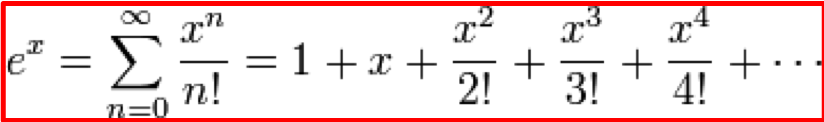
\includegraphics[width=0.5\textwidth]{images/Taylor.png}

For example, when $x = 1$:
$
e =  \sum_{n=0}^{\infty} \frac{1}{n!}
$

then:

$
e = \frac{1}{0!} +  \frac{1}{1!} + \frac{1}{2!} +  \dots
$

Write a function \texttt{my\_exp} that receives the value of $x$ as a parameter and uses an iteration to calculate the $n$-th term of the series, and adding these terms obtains an approximation to the value of $e^x$. You can use your \pythoninline{factorial} function from the previous exercise.


You can use \texttt {math.exp} as the expected result in your parameterized pytest cases (ie in your \pythoninline {@pytest.mark.parametrize} list). Remember to keep in mind that comparing floats for equality has rounding and precision problems. We can compare that the difference between what comes out of our function and the math.exp is less than, for example, $10^{-7}$.

\begin{small}
\begin{python}
def test_my_exp(tc, input, expected_output):
    assert abs(my_exp(input) - expected_output)<10**-7, "case {0}".format(tc)
\end{python}
\end{small}


\begin{howTILEd}
Insist that the students test their programs by providing them a parallel oracle and a pytest on how to use it.
\end{howTILEd}



\item Write a function to calculate the greatest common divisor (\pythoninline{gcd}) of its two parameters $x$ and $y$, which are integers and greater than 0.
%
Use Euclid's algorithm. Let $x$ e $y$ be the original values of the variables $a$ and $b$, the algorithm says:

As long as a and b are not equal, change the greater of the two for the difference between the greater and the lesser. When they have the same value, that's the \pythoninline{gcd} of $x$ and $y$.

Properties on which the Euclid algorithm is based:

\begin{itemize}
\item At the end of each iteration: \pythoninline{gcd}($x$, $y$)= \pythoninline{gcd}($a$, $b$) 
\item This property is a consequence of the mathematical property:
\begin{itemize}
\item  \pythoninline{gcd}($a$, $b$) = \pythoninline{gcd}($a - b$, $b$) when $a > b$
\item \pythoninline{gcd}($a$, $b$) = \pythoninline{gcd}($a$, $b - a$) when $b > a$ 
\end{itemize}
\item When finally $a = b$, \pythoninline{gcd}($x$, $y$) = \pythoninline{gcd}($a$, $b$)
\end{itemize}


Write pytests to test your implementation.
If we read the description of the exercise well, we see that the function does not have to work for numbers that are not greater than 0.


\begin{howTILEd}
Insist that the students test their programs by adding a line telling them to do it and make sure they read well what the function is supposed to do.
\end{howTILEd}


\item Write a function \pythoninline{gcd_3num} that calculates the greatest common divisor of more than 2 numbers. To do this, use the function \pythoninline{gcd} (greatest common divisor of 2 numbers).

Write pytests to test your implementation.

\begin{howTILEd}
Insist that the students test their programs by adding a line telling them to do it.
\end{howTILEd}

\item Write a function that, given an integer $N1$, returns another integer $N2$ that is the result of removing the first and last digit of $N1$. Note: If $N1$ has 2 digits or only one, then $N2$ must be 0. Examples of test cases that you can automate with pytest are:

\begin{longtable}{|l|l|l|}
\hline
testcase number & input ($N1$) & expected output ($N2$)  \\ \hline
1  & 42635   & 263 \\ 
2  & 23     & 0\\
3 & 5     & 0 \\
4 & 0      & 0 \\
5 & -3456  & -45 \\
\hline
\end{longtable}

\begin{howTILEd}
Insist that the students test their programs by giving them a table of test cases.
\end{howTILEd}


\item Write a function that receives a number $N$ as a parameter and generates a string with the numbers: $$1, 1, 2,
1, 2, 3, 1, 2, 3, 4, 1, 2, 3, 4, 5, . \-. . , 1, 2, 3, . . . , N $$

Examples of test cases that you can automate with pytest are:

\begin{longtable}{|l|l|l|}
\hline
testcase number & input ($N$) & expected output  \\ \hline
1  & 4   & \verb@"1, 1, 2, 1, 2, 3, 1, 2, 3, 4"@ \\ 
2  & 1   & \verb@"1"@\\
3 &  0   & \verb@""@ \\
4 &  -3  & \verb@"-1, -1, -2, -1, -2, -3"@ \\
\hline
\end{longtable}

\begin{howTILEd}
Insist that the students test their programs by giving them a table of test cases.
\end{howTILEd}

\item Write a function that receives a password as a parameter and determines its complexity, according to these rules:

\begin{itemize}
\item A very weak password contains only numbers and is less than eight characters long.

\item A weak password contains only letters and is less than eight characters long.

\item A strong password contains letters and at least one number, and is at least eight characters long.

\item A very strong password contains letters, numbers, and special characters and is at least eight characters long.

\item Passwords that are not weak or strong are normal.
\end{itemize}

Remember that in theory class we have seen the following predefined functions in Python:

- \pythoninline{isdigit}, to check if a string has digits.

- \pythoninline{isalpha} to check if a string only contains characters of the alphabet.

To test your function well, how many test cases have you run? Have you thought about both lowercase and uppercase?


\begin{howTILEd}
Insist that the students test their programs by asking them questions on what would be good test cases.
\end{howTILEd}

\end{enumerate}


\section{Lists}

\begin{enumerate}
%\setlength{\itemindent}{1.5cm}


\item Write a function that, given an integer $n$ greater than zero, returns a list of the multiples of 3 that exist between 3 and $n$. Write another function that, given an integer $n$ greater than zero, returns a list of the divisors of $n$. Test your functions with pytest, for example:

\begin{python}
@pytest.mark.parametrize('testcase, input, expected_output',[
    (1, 10, [3, 6, 9]),
    (2, 0, []),
    (3, 1, []),
    (4, -5, []),
    (5, 12, [3, 6, 9, 12]),
    (6, 3, [3])
    ])
def test_multiples_of_3(testcase, input, expected_output):
    assert multiples_of_3(input)==expected_output, 'case {0}'.format(testcase)

@pytest.mark.parametrize('testcase, input, expected_output',[
    (1, 10, [1, 2, 5, 10]),
    (2, 18, [1, 2, 3, 6, 9, 18]),
    (3, 1, [1]),
    (4, -5, []),
    (5, 12, [1, 2, 3, 4, 6, 12]),
    (6, 0, [])
    ])
def test_divisors_of(testcase, input, expected_output):
    assert divisors_of(input)==expected_output, 'case {0}'.format(testcase)
\end{python}

Now, use these functions to write a \pythoninline{main} program that asks the user for a number greater than zero through the keyboard that returns the following:

\begin{Verbatim}[frame=single]
>>> %Run 
  Type an integer greater than zero: 1
  There are no multiples of 3
>>> %Run 
  Type an integer greater than zero: 2
  There are no multiples of 3
>>> %Run 
  Type an integer greater than zero: 3
  multiple = 3, divisors of 3 = [1, 3]
>>> %Run 
  Type an integer greater than zero: 12
  multiple = 3, divisors of 3 = [1, 3]
  multiple = 6, divisors of 6 = [1, 2, 3, 6]
  multiple = 9, divisors of 9 = [1, 3, 9]
  multiple = 12, divisors of 12 = [1, 2, 3, 4, 6, 12]
>>> 
\end{Verbatim}


\item Write a function (\pythoninline{dniLetter}) that, given a DNI number, returns the letter that corresponds to it.
%
The algorithm to calculate the control letter of a DNI is the following:
\begin{itemize}
\item Find the remainder by dividing the number by 23
\item The letter is obtained using the remainder as
index of the following table:
  
  \begin{tabular}{|c|c|c|c|c|c|c|c|c|c|c|c|c|}
    \hline
    REMAINDER & 0 & 1 & 2 & 3 & 4 & 5 & 6 & 7 & 8 & 9 & 10 & 11  \\ \hline
    LETTER & T & R & W & A & G & M & Y & F & P & D & X & B  \\ \hline
  \end{tabular}
  
  \begin{tabular}{|c|c|c|c|c|c|c|c|c|c|c|c|}
    \hline
    REMAINDER & 12 & 13 & 14 & 15 & 16 & 17 & 18 & 19 & 20 & 21 & 22 \\ \hline
    LETTER & N & J & Z & S & Q & V & H & L & C & K & E  \\ \hline
  \end{tabular}
\end{itemize}


Complete the table with the number of rows you consider necessary to design your test set and run the automatic tests with pytest.\\

\begin{tabular}{|l|l|l|}
\hline
test case number & input & expected output   \\ \hline\hline
1 & \verb@                      @ & \verb@                       @\\
2 & & \\
3 & & \\
4 & & \\
5 & & \\
6 & & \\
\hline
\end{tabular}


\item Design a function that given a text string, returns the numbers that appear in the string. For example, the string `a 1, a 201, and 2 ones' contains 3 numbers: 1, 201, and 2.

\begin{Verbatim}[frame=single, label={\em example of executions}]
>>> nums_in_string("a 1, a 201 and 2 ones")
  3
>>> nums_in_string("without numbers")
  0
>>> nums_in_string("2345543")
  1
\end{Verbatim}

Write pytests to test your function in an automated way.

\item Implement a module with a \pythoninline{main} that reads a string representing a binary number from the keyboard. If any character in the string is different from 0 or 1, the program will warn the user that the entered string does not represent a binary number and will ask to read the string again. Finally, the \pythoninline{main} will display the decimal integer value of the entered binary number.

In the \pythoninline{main} you must use 2 functions that you have to define, and test with pytest:

\begin{itemize}
\item \pythoninline{check_if_is_binariy} that given a text string, it returns \pythoninline{True} if the string is composed of only 0 and 1, and if it does not, it returns \pythoninline{False}.
\item \pythoninline{convert} to convert a string in binary format (i.e. only 0 and 1) to decimal format.
\end{itemize}

What test cases would you run to test your main well?
And for the 2 functions? Implement the tests with pytest.


\item Implement a function \pythoninline{fib(n)} that returns a list with the first \pythoninline{n} numbers of Fibonacci. If \pythoninline{n == 0}, the function must return the list \pythoninline{[1]}, if \pythoninline{n == 1}, the function must return the list \pythoninline {[1,1]}. When \pythoninline{n < 1}, then start with the list \pythoninline {[1,1]} and add the next Fibonacci number by adding the previous numbers in the list.

For example by typing:

\begin{Verbatim}[frame=single]
>>> print(fib(0))
  [1]
>>> print(fib(1))
  [1, 1]
>>> print(fib(2))
  [1, 1, 2]
>>> print(fib(12))
  [1, 1, 2, 3, 5, 8, 13, 21, 34, 55, 89, 144, 233]
\end{Verbatim}

Don't forget your pytests to automate the tests!

\item Write a Python function \pythoninline{delete_negatives} that takes a list as an argument and returns the same list but without the negative elements.

\begin{Verbatim}[frame=single]
>>> borrar_negativos([0,-1,-11,2,33,-100,5])
  [2, 33, 5]
>>> borrar_negativos([-1,-11,-3])
  []
>>> borrar_negativos([4,68,111])
  [4, 68, 111]
\end{Verbatim}

Run more automated tests with pytest. Don't forget a test for the empty list and the list with 1 element.

\item Write a function (\pythoninline{maxPos}) that, given a non-empty list, returns the position where its maximum value is found.
Then complete the table below with the number of rows you see necessary to design your test set and run the automatic tests with pytest. This time it is not necessary to test the empty list, because the statement clearly says that your function only has to work for a non-empty list.\\

\begin{tabular}{|l|l|l|}
\hline
test case number & input & expected output   \\ \hline\hline
1 & \verb@                      @ & \verb@                       @\\
2 & & \\
3 & & \\
.... & & \\
\hline
\end{tabular}


\item Write a function that, given a list of words and a word, returns the number of times that word appears in the list. Then, complete the table with the number of rows that you see necessary to design your test set and run the automatic tests with pytest.\\

\begin{tabular}{|l|l|l|}
\hline
test case number & input & expected output   \\ \hline\hline
1 & \verb@                      @ & \verb@                       @\\
2 & & \\
3 & & \\
.... & & \\
\hline
\end{tabular}

\item Design a function (\pythoninline{mySplit}) that gets a string and returns a list of all its words in lowercase. The returned list must not contain repeating words.
You can't use Python's default \pythoninline {split}.
For example, with the string:

\begin{Verbatim}[frame=single]
>>> mySplit('A phrase made up of words. Another phrase with other words.')
  ['a', 'phrase', 'made', 'up', 'of', 'words', 'another', 'with', 'other']
>>> mySplit('Hi! Helloooo HI')
  ['hi', 'helloooo']
\end{Verbatim}

To design your set of tests that you have to run automatically with pytest, think about these cases:

\begin{itemize}[nosep]
    \item the string is empty
    \item the string has punctuation marks, like \verb|,;.:-¿?+*()!¡|
    \item the string ends with a point
    \item the string does not end with a point
    \item the string has numbers
    \item que the string has repeated words, but some are capitalized and some are not (for example: \pythoninline{'HEllo hello heLlo'}
    \item the string has more than 1 space between words
    \item etc.
\end{itemize}


\item Write a function that, given a list of numbers, returns another list without the odd numbers.
Then complete the table with the number of rows you see necessary to design your test set and run the automatic tests with pytest.\\

\begin{tabular}{|l|l|l|}
\hline
test case number & input & expected output   \\ \hline\hline
1 & \verb@                      @ & \verb@                       @\\
2 & & \\
3 & & \\
.... & & \\
\hline
\end{tabular}

\item Write a function that, given a list of numbers, returns another list without repeating elements. Then complete the table with the number of rows you see necessary to design your test set and run the automatic tests with pytest.\\

\begin{tabular}{|l|l|l|}
\hline
test case number & input & expected output   \\ \hline\hline
1 & \verb@                      @ & \verb@                       @\\
2 & & \\
3 & & \\
.... & & \\
\hline
\end{tabular}


\item Write a module with three functions about matrices, and their pytests: \pythoninline{sum\_of\_diagonal}, \pythoninline{create\_matrix} and \pythoninline{multiply}.

1) The first function is (\pythoninline{sum\_of\_diagonal}) that, given a $m$ matrix of integers, calculates the sum of the integers that are on the diagonal. Your function has to check that the matrix is square and does indeed have a diagonal to add. For example:

$
{\tt sum\_of\_diagonal}(
\begin{bmatrix}
    1 & 2 & 3 & 4 \\
    2 & 4 & 6 & 1 \\
    0 & 5 & 8 & 2 \\
    2 & 9 & 6 & 3 \\
\end{bmatrix})
 = 16
$, $\;\;$
$
{\tt sum\_of\_diagonal}(
\begin{bmatrix}
    1 & 5   \\
    3 & 4  \\
\end{bmatrix})
 = 5
$

Your function must pass the following tests:

\begin{small}
\begin{python}
@pytest.mark.parametrize("testcase, input, output",[
(1, [[1,2,3],[4,5,6],[7,8,9]], 15),
(2, [[1,0,1],[1,1,0],[1,1,1]], 3),
(3, [[2,0],[0,2]], 4),
(4, [[2,0],[0,2,3]], "the matrix is not square"),
(5, [], 0)]

def test_sum_of_diagonal(testcase, input, output):
    assert sum_of_diagonal(input) == output,\
           "case {0}".format(testcase)
\end{python}
\end{small}

2) Next, we write a function (\pythoninline{create\_matrix}) that, given two numbers $n$ and $m$, returns a list that represents a matrix with $n$ rows and $m$ columns, all values being 0.

$
{\tt create\_matrix}(3,4) = 
\begin{bmatrix}
    0 & 0 & 0 & 0 \\
    0 & 0 & 0 & 0 \\
    0 & 0 & 0 & 0 \\
\end{bmatrix})
$

Design a set of test cases and automate them with the pytest.

3) The third function is for (\pythoninline{multiply}). Given two matrices $m_1$ and $m_2$, returns $m_1 \times m_2$. Remember\footnote{\url{https://es.wikipedia.org/wiki/Multiplicación_de_matrices}}
that we can only multiply 2 matrices if the number of columns in the $m_1$ matrix is equal to the number of rows in the $m_2$ matrix.\\

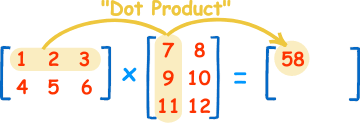
\includegraphics[width=0.5\textwidth]{images/mult-matrix.png}

Your function must pass the following tests:

\begin{small}
\begin{python}
@pytest.mark.parametrize("testcase, input1, input2, output",[
(1, [[12,7,3], 
     [4, 5,6], 
     [7, 8,9]],
    [[5,8,1,2],
     [6,7,3,0],
     [4,5,9,1]],
    [[114, 160,  60, 27], 
     [ 74,  97,  73, 14], 
     [119, 157, 112, 23]]
),
(2, [[12,7,3, 0], 
     [ 4,5,6,12], 
     [ 6,7,8, 9]
    ],
    [[8,5,8,1,2],
     [6,9,7,3,0],
     [4,5,9,1,0],
     [4,5,9,1,0]
    ],
    [[150, 138, 172, 36, 24], 
     [134, 155, 229, 37, 8], 
     [158, 178, 250, 44, 12]
    ]
),
(3, [], [], []
),
(4,[[]],[[]], "they cannot be multiplied"
),
(5, [[]],[[[]]], "they cannot be multiplied"
),
(6, [[[]]],[[]], [[]]
)
])

def test_multiply(testcase, input1, input2, output):
    assert multiply(input1, input2) == output, 
           "case {0}".format(testcase)
\end{python}
\end{small}

\end{enumerate}


\section{Text files}

\begin{enumerate}
%\setlength{\itemindent}{1.5cm}

\item Make an interactive program in Python that asks for the number of people to store, and from each one of them asks for the following data by keyboard: day, month and year of birth (integers) and name of the person (String). Then it must store it in a file called \verb|"dates.txt"| with the following format:


\begin{Verbatim}[frame=single, label={\em dates.txt}]
    12 03 1996 | Hira Sadler
    16 05 1997 | Roman Connelly
    08 10 1976 | Alexandre Bullock
    04 03 2010 | Tracy Kendall
\end{Verbatim}

The above file has resulted from the following interactive session:\\

\begin{Verbatim}[frame=single, label={\em example with 4 people}]
>>> %Run 
  Number of people to store: 4
  
  Give the data for person 1:
  Day: 12
  Month: 3
  Year: 1996
  Name: Hira Sadler
  
  Give the data for person 2:
  Day: 16
  Month: 5
  Year: 1997
  Name: Roman Connelly
  
  Give the data for person 3:
  Day: 8
  Month: 10
  Year: 1976
  Name: Alexandre Bullock
  
  Give the data for person 4:
  Day: 4
  Month: 3
  Year: 2010
  Name: Tracy Kendall
  
  The file "dates.txt" has been generated.
>>>
\end{Verbatim}



\item From the previous exercise, make a program that reads the file \verb|"dates.txt"| and tells us how many people were born in May. In the example above, there is only one person who was born in May. To test your program well, make sure that you also test it with different files \verb|"dates.txt"|:

\begin{itemize}
    \item a file \verb|"dates.txt"| which has no one born in May
    \item a file \verb|"dates.txt"| which has more than one person born in May
\end{itemize}


\item We have the following format for a text file:\\

\begin{Verbatim}[frame=single, label={\em threegrades.txt}]
    23 2.5 3.0 1.1
    34 2.0 1.0 1.0
    17 1.0 1.0 1.1
    450 4.0 2.1 2.2
    55 4.0 4.0 2.0
\end{Verbatim}

In each line we have:
\begin{itemize}
    \item the student's file number, which is an integer
    \item the grade of the first partial, a real value
    \item the grade of the second partial, a real value
    \item the attendance grade, a real value
\end{itemize}



Write a function \pythoninline{calculate\_notes} in Python that receives as a parameter the name of a text file that has the format as \verb|tresnotas.txt|, and writes on the screen the total number of students and how many of them have passed. A student will be deemed to have passed when the sum of his three grades is greater than or equal to 5.\\

\begin{Verbatim}[frame=single, label={\em example of calling the function calculate\_grades}]
>>> calculate_grades("threegrades.txt")
  number of students: 5
  number of students who have passed: 3
>>> 
\end{Verbatim}


\item \label{generate_files}
Write a Python program that allows you to generate a certain number of files with a random number (between 1 and 10) of random real numbers (between 1.00 and 200.00). The numbers must be aligned to the right and with 2 decimal places. You can import \pythoninline{random} and use \pythoninline{randint} to randomly generate integers, and \pythoninline{uniform} to randomly generate real numbers.

Your program:

\begin{itemize}
    \item first it must ask the user for the number of files he wants to generate
    \item then it asks for the name to use as the base of the generated files. For example, if the user wants 5 files with base name \texttt{file}, the program will generate the files \texttt{file1.txt}, \texttt{file2.txt}, \dots, \texttt{file5.txt}.
\end{itemize}

For example:

\begin{Verbatim}[frame=single, label={\em interactive session example}]
>>> %Run 
  How many files?: 4
  What is the base name?: file
>>> 
\end{Verbatim}

It can generate for example:

\begin{tabular}{p{3cm}p{3cm}p{3cm}p{3cm}}

\begin{Verbatim}[frame=single, label={\em file1.txt}]
 133.25 
 159.93 
 162.02 
  23.26 
 147.50 
\end{Verbatim}
&
\begin{Verbatim}[frame=single, label={\em file2.txt}]
  29.92 
 199.44 
 158.01 
\end{Verbatim}
&
\begin{Verbatim}[frame=single, label={\em file3.txt}]
  50.08 
  59.34 
 109.88 
 153.48 
 195.16 
  51.95 
  86.55 
 153.28 
\end{Verbatim}
&
\begin{Verbatim}[frame=single, label={\em file4.txt}]
   6.64 
 136.33 
  32.02 
  56.16 
  97.67 
 160.56 
\end{Verbatim}
\end{tabular}

\item Write a function \pythoninline{calculate\_variance} in Python that receives the name of a file and reads a number of real numbers from this file, storing them in a list. Then it shows the variance of these data on the screen. The variance is calculated as the sum of the squared differences between each element in the list, v[i], and the mean, all divided by the number of elements (N):
\begin{equation}
  w = \frac{\sum_{i=1}{n} (x[i]-mean)^{2}}{N}
\end{equation}

For example, imagine we have:

\begin{Verbatim}[frame=single, label={\em numbers.txt}]
   6.64 
 136.33 
  32.02 
  56.16 
  97.67 
 160.56 
\end{Verbatim}


\begin{Verbatim}[frame=single, label={\em function call example}]
>>> calculate_variance("numbers.txt")
  3035.443822222222
\end{Verbatim}


To test your function we are going to use Exercise \ref{generate_files} to generate a number of files (eg 5 files \texttt{numbers1.txt}, \texttt{numbers2.txt}, \texttt{numbers3.txt}, \texttt{numbers4.txt} and \texttt{numbers5.txt}).

Then we go to \url{https://www.calculatorsoup.com/calculators/statistics/variance-calculator.php} to calculate the variance of the data in these 5 files. In this way we have the expected results of our function.

Then finish the following pytest code to run your tests automatically:


\begin{python}
import pytest

@pytest.mark.parametrize("testcase, f_input, expected_output",[
(1, "numbers1.txt",  3713.1622346939),
(2, "numbers2.txt", ...
(3, 
(4,
(5,
])

def test_calculate_variance(testcase, f_input, expected_output):
    assert abs(calculate_variance(f_input) - expected_output) < 10**-7 ,\
           "case {0}".format(testcase)
\end{python}

Remember to keep in mind that comparing floats for equality has rounding and precision problems. That is why we must compare that the difference between what comes out of our function and what we expect is less than, for example, $10^{-7}$.




\item Implement a \pythoninline{calculate\_IVA} function in Python that receives a name from a text file (for example \texttt{data.txt}) where the prices without IVA of some items are found. Your function must read these prices, apply IVA (21 $\%$) to them and save the values with VAT in a file named \texttt{data\_IVA.txt}. The data in \texttt{data\_IVA.txt} must be aligned to the right and with 2 decimal places. In addition to generating the file, your function has to return the name of the generated file.

For example: \pythoninline{calculate\_IVA("data1.txt")} returns the string \texttt{"data1\_IVA.txt"} which is the name of the generated file:

\begin{tabular}{p{3cm}p{2cm}p{9cm}}

\begin{Verbatim}[frame=single, label={\em data1.txt}]
 12.05
  6.70
123.10
333.33
 25.50
100
  9.95    
\end{Verbatim}
&
\begin{Verbatim}
 
 
 
generates
 
 
   
\end{Verbatim} 
&

\begin{Verbatim}[frame=single, label= the expected content of file {\em data1\_IVA.txt}]
  14.58 
   8.11 
 148.95 
 403.33 
  30.86 
 121.00 
  12.04 
\end{Verbatim}
\end{tabular}


\item To test a function like \pythoninline{calculate\_IVA}, which generates a file, you have to open the file it has generated to check that it has the content you expected. For example, if you used the file \texttt{data1.txt} as input, you would expect a file with name \texttt{data1\_IVA.txt} that has the content as shown in the example above.

Doing that manually is tedious. Imagine doing it for 10 data files, from \texttt{data1.txt} to \texttt{data10.txt}, that we can generate for example with the Exercise \ref{generate_files}.
%
We would have to manually generate the 10 files from \texttt{data1\_IVA.txt} to \texttt{data10\_IVA.txt}, with \pythoninline{calculate\_IVA}, and then open them one by one to check their content to see if it is what we expect.

We can automate it with pytest. However, the output of the function is not just a value as we have seen so far. The output of the \pythoninline{calculate\_IVA} function is a file. So the expected output can also be a file, and the test simply compares that what comes out is equal to what we expect!

For that, we must create 10 files only once where we define the expected outputs of our tests: from \textttt{expected\_output\_data1\_IVA.txt} to \textttt{expected\_output\_datos10\_IVA.txt}. Then we create a pytest like the one below:

{\footnotesize
\begin{python}
@pytest.mark.parametrize("testcase, f_input, f_expected_output",[
(1,  "data1.txt",  "expected_output_data1_IVA.txt"),
(2,  "data2.txt",  "expected_output_data2_IVA.txt"),
(3,  "data3.txt",  "expected_output_data3_IVA.txt"),
(4,  "data4.txt",  "expected_output_data4_IVA.txt"),
(5,  "data5.txt",  "expected_output_data5_IVA.txt"),
(6,  "data6.txt",  "expected_output_data6_IVA.txt"),
(7,  "data7.txt",  "expected_output_data7_IVA.txt"),
(8,  "data8.txt",  "expected_output_data8_IVA.txt"),
(9,  "data9.txt",  "expected_output_data9_IVA.txt"),
(10, "data10.txt", "expected_output_data10_IVA.txt"),
])

def test_calculate_IVA(testcase, f_input, f_expected_output):
    
    f_output = calculate_IVA(f_input)

    assert (open(f_output).read() == open(f_expected_output).read()),\
           "case {0}".format(testcase)
\end{python}
}

NOTE: To compare the files we have used \pythoninline{read} because the size of the files that we are handling here is very small.

\item Write Python code that prompts the user for a 4-character word and creates the following heart in a heart.txt file.\\

\begin{verbatim}
    HART        HART
 HART HART  HART HART
HART     HART     HART
HART              HART
 HART            HART
  HART          HART
    HART      HART
      HART  HART
         HART
\end{verbatim}

\end{enumerate}


\section{Dictionaries}

\begin{enumerate}
%\setlength{\itemindent}{1.5cm}

\item Write a program that stores in a variable the next dictionary:

\verb!{'Euro':'!\euro', 'Dollar':'
\verb!$', 'Yen':'!\yen
\verb!'},! 

It should ask the user for a currency and display its symbol or a warning message if the currency is not in the dictionary.

\begin{Verbatim}[frame=single, label = {\em example test runs}]
>>> %Run 
  Enter a currency: Euro
  €
>>> %Run 
  Enter a currency: Dollar
  $
>>> %Run 
  Enter a currency: Wow
  That currency is not in the dictionary
\end{Verbatim}


%\solution{
%dictionary = {'Euro':'€' , 'Dolar':'$', 'Yen':'¥'}
%currency = input("Enter a currency: ")
%print(dictionary.get(currency.title(), "That currency is not in the dictionary"))
%}

\item Write a function called \pythoninline{text\_to\_dic} that receives a text as an argument. It must create and return a dictionary where the keys are the words in the text, and their values are the number of occurrences of each of these in the text.

Use the function you just wrote to define a function called \pythoninline{file\_to\_dic} that receives the name of a text file and returns a dictionary where the keys are the words of the text in the file and its values the number of appearances of each of these in the text of the file.

Don't forget your documentation and pytests. To facilitate the creation of your test cases, in Poliformat there is a \texttt{text.txt} file that contains the following dictionary:


\begin{python}
{'Es': 13, 
 'un': 52, 
 'hecho': 13, 
 'hace': 11, 
 'tiempo': 8, 
 'que': 23, 
 'lector': 9, 
 'mira': 13, 
 'el': 11, 
 'de': 26, 
 'texto': 13, 
 'sitio': 11, 
 'mientras': 9, 
 'que.': 3, 
 'contenido': 10, 
 'mira.': 10
}
\end{python}
 
A histogram is a graphical representation of a variable in the form of bars, where the area of each bar is proportional to the frequency of the values represented. They are used to obtain a general "first view" or panorama of the distribution of the population, or of the sample, regarding a characteristic, quantitative and continuous (such as length or weight) (see \url{https://es.wikipedia.org/wiki/Histograma}).

Write a function \pythoninline{ascii\_histogram} that receives as an argument a dictionary with keys of type string and values of type int, and returns an ASCII histogram that uses the Python output format. An example is below:

\begin{Verbatim}[frame=single]
>>> ascii_histogram(file_to_dic("text.txt"))
             Es +++++++++++++
             un ++++++++++++++++++++++++++++++++++++++++++++++++++++
          hecho +++++++++++++
           hace +++++++++++
         tiempo ++++++++
            que +++++++++++++++++++++++
         lector +++++++++
           mira +++++++++++++
             el +++++++++++
             de ++++++++++++++++++++++++++
          texto +++++++++++++
          sitio +++++++++++
       mientras +++++++++
           que. +++
      contenido ++++++++++
          mira. ++++++++++
\end{Verbatim}

Create a test case to test the function \pythoninline{ascii\_histogram} that returns as expected result:

\begin{Verbatim}[frame=single]
>>> ascii_histogram(dic)
              0 
              1 +
              2 ++
              3 +++
              4 ++++
              5 +++++
              6 ++++++
              7 +++++
              8 ++++
              9 +++
             10 ++
             11 +
\end{Verbatim}

\item Write a program that creates a dictionary that simulates a shopping cart. The program must ask for the item and its price, and add the pair to the dictionary, until the user decides to finish. Then, the shopping list and the total cost should be displayed, as in the following example:
\begin{small}
\begin{Verbatim}[frame=single]{\em example test run}
>>> %Run 
  Enter a product: beer
  Enter its price: 1.50
  
  Do you want to continue? (Y/N): Y
  Enter a product: wine
  Enter its price: 4.50
  
  Do you want to continue? (Y/N): Y
  Enter a product: seed pack
  Enter its price: 1.00
  
  Do you want to continue? (Y/N): Y
  Enter a product: fruit
  Enter its price: 8
  
  Do you want to continue? (Y/N): N
  
  Product        Price
  --------------------
  beer           1.50€
  wine           4.50€
  seed pack      1.00€
  fruit          8.00€
  --------------------
  Total         15.00€
\end{Verbatim}
\end{small}

You can assume that the user only adds 1 sample of each product. Your tests can be run through the shell manually.

\solucion{
basket = {}
more = 'Si'
while more == 'Si':
    item = input('Enter a product: ')
    price = float(input('Enter its price: '))
    basket[item] = price
    more = input('Do you want to continue? (Y/N): ')
cost = 0
print('Shopping list')
for item, price in basket.items():
    print(item, '\t', price)
    cost += price
print('Total: ', price)
}


\item In the Scrabble game, each letter has scores associated with them. The total score
of a word is the sum of its letter scores. The most common letters are worth less points, while the less common letters are worth more points. We are going to use a dictionary that maps from letters to point values. The points associated with each letter are shown below:

\begin{python}
points = {"A": 1, "B": 3, "C": 3, "D": 2, "E": 1, "F": 4,
          "G": 2, "H": 4, "I": 1, "J": 2, "K": 5, "L": 1,
          "M": 3, "N": 1, "O": 1, "P": 3, "Q": 10, "R": 1,
          "S": 1, "T": 1, "U": 1, "V": 4, "W": 4, "X": 8,
          "Y": 4, "Z": 10
          }
\end{python}

Write a function that calculates and displays the Scrabble score for a given word.
Use the dictionary to calculate the score.

The Scrabble board includes some cells that multiply the value of a letter or the value of a whole word. We will ignore these squares in this exercise.

Write pytests to test your function, for example for the following test cases:

\begin{longtable}{|l|l|l|}
\hline
testcase number & input & expected output   \\ \hline
1  &  \verb|''|  & 0 \\ 
2  &  \verb|'Hello!'|    & 8\\
3 &  \verb|'zzz'|    &  30\\
4 &  \verb|'Surprise'|     & 10 \\
5 & \verb|'1234'|  & 0 \\
6 & \verb|'And with spaces?'|  & 24 \\
\hline
\end{longtable}


\item In this exercise you must simulate 1000 rolls of two dice. First, write a function called \pythoninline{twoDice()}, which simulates throwing 2 six-sided dice. Your function won't take any parameter and will return the total that was rolled on two dice as the only result.

Then, write a main program that uses this function to simulate the rolling of two dice 1000 times. As your program runs, you have to count the number of times each total occurs and save it to a dictionary. Then it should display a table that summarizes this data.

On the one hand you have to show the percentage expected by the probability theory for each total:

\begin{python}
expected_probability = {2: 1/36, 3: 2/36, 4: 3/36, 5: 4/36, 
                         6: 5/36, 7: 6/36, 8: 5/36, 9: 4/36, 
                         10: 3/36, 11: 2/36, 12: 1/36
                        }
\end{python}

The frequency of each total as a percentage of the number of dice rolls made. The output is shown below.

\begin{verbatim}
Total   Simulated Percentage     Expected Percentage
----------------------------------------------------
6       14.20                    13.89
8       13.70                    13.89
3       5.50                     5.56
7       18.00                    16.67
2       2.40                     2.78
10      8.00                     8.33
5       10.70                    11.11
9       11.50                    11.11
11      6.30                     5.56
4       7.40                     8.33
12      2.30                     2.78
\end{verbatim}


\item Morse code is a coding scheme that uses hyphens and dots to represent digits and letters. In this exercise, we are going to write a program that uses a dictionary to store the mapping between these symbols and Morse code. Use a dot to represent a Morse dot, and
a hyphens to represent a Morse hyphens. The mapping of characters to hyphens and dots is
shown in the table below:

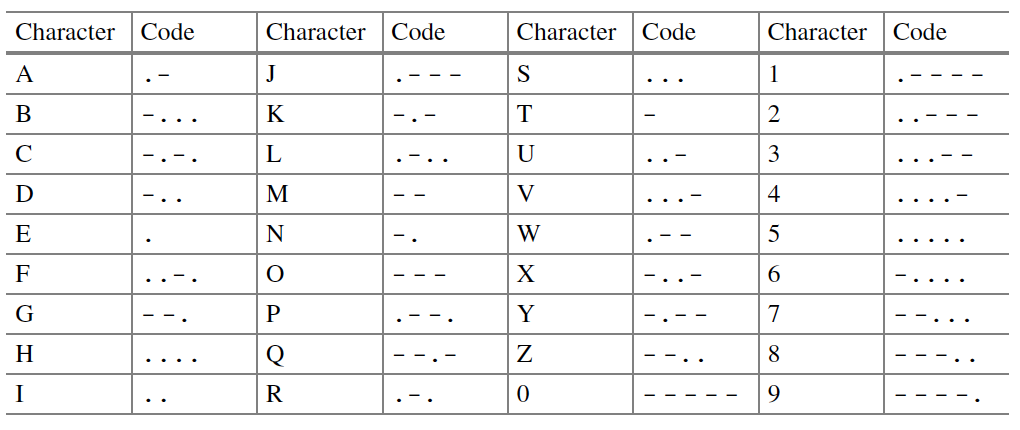
\includegraphics[width=14cm]{images/morse.png}

First, you have to write a function that translates words written in capitalized English into Morse code. The function must ignore any characters in the word that are not listed in the table above.

After testing the function well, you have to write a program called \pythoninline{main} that calls this function to translate a message that asks the user. The user's message can consist of more than one word separated by a space.

For example, if you are a user, type the message \pythoninline {Hello, World!} and your program must return the following Morse code:

\begin{verbatim}
.... . .-.. .-.. --- .-- --- .-. .-.. -..
\end{verbatim}

 
\item Write a program that allows you to manage the customer data of a company. This should be stored in a dictionary in which:

\begin{itemize}
\item the key of each client will be their NIF, and
\item the value will be another dictionary with the customer's data (name, address, phone, email, VIP), where the customer will have the value True if is a VIP customer.
\end{itemize}

The program should ask the user for an option from the following menu:

\begin{verbatim}
(1) Add customer,
(2) Delete customer,
(3) Show client,
(4) List all clients,
(5) List VIP clients,
(6) Finish.
\end{verbatim}

Depending on the option chosen, the program must to do the following:
\begin{description}
    \item[\verb|(1)|] Ask for the customer's data, create a dictionary with the that information and add it to the database. If a client with the same NIF already exists, a message must be displayed indicating it.
    \item[\verb|(2)|] Ask for the customer's NIF and delete their data from the database. If a client with this same NIF does not exist, a message must be displayed indicating it.
    \item[\verb|(3)|] Ask for the customer's NIF and show their data. If a client with this same NIF does not exist, a message must be displayed indicating it.
    \item[\verb|(4)|] Show the list of all the clients in the database, with their NIF and name.
    \item[\verb|(5)|] Show the list of the VIP clients from the database, with their NIF and name.
    \item[\verb|(6)|] End the program.
\end{description}

You have to test your program well manually, thinking for each option which would be good test cases to ensure quality testing. For example, you can do the following interactions:

\begin{description}
\item[-] add a VIP client
\item[-] check that it has been added correctly, by using the options \verb|(3)|, \verb|(4)| and \verb|(5)|
\item[-] add a non-VIP customer
\item[-] check that it has been added correctly, by using the options \verb|(3)|, \verb|(4)| and \verb|(5)|
\item[-] try to add another client with the same NIF, and check that your program does not allow it by giving a message
\item[-] add 3 more clients (1 VIP and 2 non-VIP)
\item[-] try to delete a client that does not exist and check that your program shows the corresponding message
\item[-] remove a customer that exists
\item[-] check that it has been deleted correctly, by using the options \verb|(3)|, \verb|(4)| y \verb|(5)|
\item[-] end the program with \verb|(6)|
\end{description}


\solucion{
def enterData(customers):
    data_nif = input('Enter the customer's NIF: ')
    data_name = input('Enter the customer's name: ')
    data_address = input('Enter the customer's address: ')
    data_phone = input('Enter the customer's phone number: ')
    data_email = input('Enter the customer's email: ')
    data_vip = input('Is a VIP customer (Y/N)?')
    customer = {'name':data_name, 'address':data_address, 'phone':data_phone, 'email':data_email, 'vip':data_vip=='Y'}
    customers[nif] = customer
    

def deleteCustomer(customers):
    nif = input('Enter the customer's NIF: ')
    if nif in customers:
        del customers[nif]
    else:
        print('There is no client with the nif ', nif)    

def showCustomer(customers):
    nif = input('Enter the customer's NIF: ')
    if nif in customers:
        print('NIF:', nif)
        for key, value in customers[nif].items():
            print(key.title() + ':', value)
    else:
        print('There is no client with the nif ', nif)
        
def listCustomers(customers):
    print('List of customers')
    for key, value in customers.items():
        print(key, value['name'])
        
def listVIPCustomers(customers):
    print('List of VIP customers')
    for key, value in customers.items():
        if value['vip']:
            print(key, value['nombre'])

def main():
    customers = {}
    option = ''

    while option != '6':
        if option == '1':
            enterData(customers)
        if option == '2':
            deleteCustomer(customers)
        if option == '3':
            showCustomer(customers)
        if option == '4':
            listCustomers(customers)
        if option == '5':
            listVIPCustomers(customers)
        option = input('Option menu\n(1) Add customer\n(2) \ Delete customer\n(3) Show customer\n(4) List customers\n(5)\
       List VIP customers\n(6) Finish\n Choose an option:')
        
if __name__=='__main__':
    main()
    
}


\item The problem with the previous exercise is that each time the program is launched, the data would have to be entered again. To avoid this, we are going to create two new options that allow us to use files as backup copies of the data in the dictionary. The menu for the user with the options will be as shown below:

\begin{verbatim}
(1) Add customer,
(2) Delete customer,
(3) Show client,
(4) List all clients,
(5) List VIP clients,
(6) Save to file,
(7) Read data from file,
(8) Finish.
\end{verbatim}


The option \verb|(6)| will store the data in a file. Selecting this option will save the current dictionary data in the customer.txt file in the following format:

nif; name; address; telephone; email; vip
for example:
\begin{verbatim}
1234;Michael Myers;2704 Hickman Street;203-355-7551;mm@f.com;True
2345;Marilyn Scott;2834 Washington Street;361-346-8703:ms@f.com:False
\end{verbatim}

The option \verb|(7)| will do the opposite operation. It will read the data from the customer.txt file and store it in the dictionary (removing all previous data from the dictionary).

Now, the option to terminate will be the \verb|(8)|.

To test your program, run the tests from the previous exercise, but before ending the program choose the option \verb|(7)|. Then, open the saved file to check that the content matches the clients.



\end{enumerate}


\section{Tuples and sets}


\begin{enumerate}
%\setlength{\itemindent}{1.5cm}

\item Write a \pythoninline{odd_sum} function that takes a list or tuple of numbers. It should return a two-element tuple, containing (respectively) the sum of the even-indexed numbers and the sum of the odd-numbered numbers. Example:

\begin{Verbatim}[frame=single, label={\em tests example}]
>>> odd_even_sum([2,4,6,1,12,3,4])
  (24, 8)
>>> odd_even_sum([0,2,4,6,1,12,3,4])
  (8, 24)
>>> odd_even_sum((1,2,1,2,1,2))
  (3, 6)
>>> odd_even_sum((2,1,2,1,2,1,2))
  (8, 3)
>>> odd_even_sum(())
  (0, 0)
>>> odd_even_sum([])
  (0, 0)
\end{Verbatim}


\item \pythoninline{zip} is a function that is predefined in Python. It takes two or more sequences and intersperses them. The name of the function refers to a zipper, since it intersperses two rows of teeth.

This example zips a string and a list:

\begin{Verbatim}[frame=single]
>>> s = 'abc'
>>> t = [0, 1, 2]
>>> zip(s, t)
<zip object at 0x7f7d0a9e7c48>
\end{Verbatim}

The result is a {\bf zip object} that contains pairs that can be iterated over. The most common use of {\tt zip} is in a {\tt for} loop:

\begin{Verbatim}[frame=single]
>>> for pair in zip(s, t):
...     print(pair)
...
('a', 0)
('b', 1)
('c', 2)
\end{Verbatim}
%

We are going to write a \pythoninline{my_zip} function that does not return a zip object, but directly the list with the tuples. You can assume that the two sequences it receives have the same number of elements:

\begin{Verbatim}[frame=single]
>>> s = 'abc'
>>> t = [0, 1, 2]
>>> mi_zip(s,t)
[('a', 0), ('b', 1), ('c', 2)]
>>> s = (1,2,3)
>>> t = [4,5,6]
>>> mi_zip(s,t)
[(1, 4), (2, 5), (3, 6)]
\end{Verbatim}

Don't forget to test your function with pytests.


\item Write a \pythoninline{tuple_inter} function that receives two sets. The function must return a tuple that contains the intersection of the two sets and the result of erasing the intersection in the first set.

For example you can test your function with:

\begin{Verbatim}[frame=single]
>>> firstSet  = {23, 42, 65, 57, 78, 83, 29}
>>> secondSet = {57, 83, 29, 67, 73, 43, 48}

>>> tuple_inter(firstSet, secondSet)
  ({57, 83, 29}, {65, 42, 78, 23})
>>> tuple_inter(firstSet, firstSet)
  ({65, 83, 23, 57, 42, 29, 78}, set())
>>> tuple_inter(set(), set())
  (set(), set())
\end{Verbatim}


\solucion{
firstSet  = {23, 42, 65, 57, 78, 83, 29}
secondSet = {57, 83, 29, 67, 73, 43, 48}

print("First Set ", firstSet)
print("Second Set ", secondSet)

intersection = firstSet.intersection(secondSet)
print("Intersection is ", intersection)
for item in intersection:
  firstSet.remove(item)

print("First Set after removing common element ", firstSet)

}

\item A common use of tuples is as records.
And of course, displaying those records in a table is a standard thing for programs to do. In this exercise, we'll do a bit of both: reading a list of tuples and displaying them
in table format for the user.

Imagine that we organize a conference on testing and we know from each speaker her name and the time he needs to travel to the conference venue.

\begin{python}
speakers = [('Jeff', 'Offutt', 7.85),
            ('James', 'Bach', 3.626),
            ('Lisa', 'Crispin', 10.603)
          ]
\end{python}

Write a \pythoninline{format_sort_records} function in Python that allows scheduling and returns the following table:

\begin{Verbatim}
James      Bach        3.63
Jeff       Offutt      7.85
Lisa       Crispin    10.60
\end{Verbatim}

This trip planner does not need the level of precision that the entry provides; it is enough for us to have two digits after the decimal point. Also note that the last name is printed after the first name, followed by a decimal-aligned indication of how long each proponent will take to arrive in increasing order. Each name must be printed in a 10-character field, and the time must be printed in a 5-character field, with a padding space character between each of the columns.


\item Write a function that receives a text string and says whether it only has unique characters or not. This function should return True if it has no repeating characters and False otherwise. Write a pytest using the following parameterization:

\begin{python}
@pytest.mark.parametrize('testcase, input, expected_output',[
    (1, 'Hello', True),
    (2, 'HelloO', False),
    (3, '', True),
    (4, 'cC', False),
    (5, '0123', True),
    (6, '33&44', False),
    (7, '!+&/', True),
    (8, '!++&/', False),
    ])
\end{python}

\solucion{
def is_unique(given_string):
    #creating an empty set
    chars_set = set()
    for char in given_string:
        #if char already in set its duplicate
        if char in chars_set:
            return False
        else:
            #char not in set, add it
            chars_set.add(char)
    #if no duplicates
    return True
    }
    

\item A famous syllogism says:

All humans are mortal.

Socrates is human.

Therefore Socrates is mortal.

In the following code, you will see multiple sets. The first contains all things (I know some are missing, but consider it complete for this problem). The second is a set of all people (assuming that the first set is really complete). The third contains everything that is mortal (again, assuming that is complete).

\begin{python}
todas = { "Socrates", "Plato", "Eratosthenes", "Zeus", "Hera",
          "Athene", "Acropolis", "Cat", "Dog" }
personas = { "Socrates", "Plato", "Eratosthenes" }
mortales = { "Socrates", "Plato", "Eratosthenes", "Cat", "Dog" }
\end{python}


Use the set operators and their methods to show that it is true that:

a) all humans are mortal,

b) Socrates is human and

c) Socrates is mortal.

(d) there are mortal things that are not human, and

(e) there are things that are not mortal.


\item Write a program that generates three sets of numbers between 1 and 1000:

the first set consists of all numbers that are divisible by 3,

the second consists of all numbers that are divisible by 7, and

the third consists of all numbers that are divisible by 11.

Then, produce sets of all numbers between 1 and 1000 that are

(a) divisible by both 3, 7, and 11,

(b) that are divisible by 3 and 7, but not by 11, and

(c) that are neither divisible by 3, nor by 7, nor by 11.



\item Write a \pythoninline{generate_eratosthenes} function that, using the Sieve of Eratosthenes \footnote{\url{https://en.wikipedia.org/wiki/Sieve_of_Eratosthenes}}, obtains the prime numbers between 2 and 120. The algorithm is based on having in a set the numbers between 2 and 120, and then eliminate from that set the multiples of 2, then those of 3, then those of 5, and so on. Pseudocode would be as can be seen below:
\begin{verbatim}
Create a set and initialize it with the numbers between 2 and 120
Initialize p to 2
As long as p is between 2 and 120
    As long as p is not within the set
        increase p
    Initialize k to 2 * p
    As long as k is less than 120
        Eliminate k from the set
        Update k to k + p
    Increase p
\end{verbatim}
\solucion{
numbers=set(range(2,120))
p = 2
while p < 120:
    while p not in numbers:
        p = p + 1
    k = 2 * p
    while k < 120:
        numbers.discard(k)
        k = k + p
    p = p + 1

print("the prime numbers are: ")
print(numbers)
}

To test your function, you can compare the numbers you obtain with those that appear below:

\animategraphics[height=2.8in,autoplay]{1}{animated_imgs/eratosh-}{0}{39}

\end{enumerate}

\printbibliography

\end{document}



